% Springer LNCS template — Quantum NLP report
% Build:  pdflatex main && bibtex main && pdflatex main && pdflatex main
% Or:     make

\documentclass[runningheads]{llncs}

\usepackage[T1]{fontenc}
\usepackage[utf8]{inputenc}
\usepackage{graphicx}
\usepackage{amsmath, amssymb}
\usepackage{booktabs}
\usepackage{array}
\usepackage{multirow}
\usepackage{hyperref}
\usepackage[capitalize]{cleveref}
\usepackage{xcolor}
\usepackage{float}
\usepackage{listings}
\usepackage{tikz}
\usetikzlibrary{positioning,arrows.meta,shapes.geometric}
\usepackage{longtable}
\usepackage{lscape}

% Inline code style
\lstset{
  basicstyle=\ttfamily\footnotesize,
  breaklines=true,
  frame=single,
  framesep=4pt,
}

% Pending-content highlighting (remove before submission)
\newcommand{\TBD}[1]{\textcolor{red}{\textbf{[TBD: #1]}}}

\hypersetup{
  colorlinks=true,
  linkcolor=blue!50!black,
  citecolor=green!50!black,
  urlcolor=blue!70!black,
}

%-----------------------------------------------------------------------
\begin{document}

\title{Quantum Sentiment Classification with DisCoCat: A Controlled Empirical Study on a Short Phrase SST-2 Subset}

\titlerunning{Quantum Sentiment Classification with DisCoCat on a Short Phrase SST-2 Subset}

\author{
  Nhat-Linh Do\inst{1}\thanks{Corresponding author.} \and
  Quang-Thai Le\inst{1} \and
  Minh-Tan Tran-Huynh\inst{2}
}

\authorrunning{N.-L. Do et al.}

\institute{
  Faculty of Business Data Science, Banking University of Ho Chi Minh City, Vietnam \\
  \email{\{linh.do,thailq\}@hub.edu.vn}
  \and
  Faculty of Management Information Systems, Banking University of Ho Chi Minh City, Vietnam \\
  \email{tanthm@hub.edu.vn}
}

\maketitle

%-----------------------------------------------------------------------
\begin{abstract}
We investigate the application of Distributional Compositional
Categorical (DisCoCat) models with variational quantum circuits to
binary sentiment classification on short phrases (2--5 tokens) drawn
from the Stanford Sentiment Treebank (SST-2). Each phrase is converted
into a DisCoCat string diagram using the \texttt{lambeq} library,
parameterised by a quantum ansatz, and trained on the \texttt{PennyLane}
simulator. A controlled experimental grid of 60 quantum runs is
conducted, spanning two diagram readers (Spiders, Cups), two ansatz
families (IQP, Sim14), three circuit depths and five random seeds.
Three classical baselines (Logistic Regression with TF--IDF bigrams,
Logistic Regression with averaged GloVe-50d embeddings, and a
single-layer bidirectional LSTM) are evaluated on the same balanced
\(5{,}000/400/400\) split.

On this short-phrase subset, the Spiders reader (which attains
identical accuracy across all six ansatz--depth configurations, as
documented below) achieves \(92.05\% \pm 0.64\%\) test accuracy using
only \(2{,}940\) trainable parameters. Two separate comparisons are
reported. Against the dense sequence baseline (BiLSTM,
\(91.83\% \pm 0.42\%\), \(82{,}369\) parameters), the Spiders model
is statistically indistinguishable (McNemar \(p = 0.60\)) at
\(28\times\) fewer parameters. Against the sparse linear baseline
(LR + TF--IDF, \(94.25\%\), \(2{,}829\) parameters), the picture is
reversed: the linear model is both leaner and 2.2 percentage points
more accurate; this gap reaches raw McNemar \(p = 0.045\) but is not
significant after Holm--Bonferroni adjustment over the family of
\(16\) comparisons (\(p_{\text{Holm}} = 0.39\)). The Spiders result
should be read as a property of the compositional DisCoCat embedding
into single-qubit unitaries rather than as evidence of a general
quantum advantage; the entangling Cups + Sim14 variant matches but
does not exceed it, and the linear TF--IDF baseline remains the most
parameter-efficient model overall on the studied subset. Two
methodologically informative observations are reported. First, with
single-qubit atomic types the Spiders reader becomes representationally
degenerate: every ansatz--depth combination reduces to the same
single-qubit unitary, and all six Spiders configurations attain
identical accuracy. Second, the Cups reader combined with the IQP
ansatz exhibits a reproducible barren-plateau-like collapse at depth two
(\(62.8\%\) across all five seeds), which persists despite the use of a
\texttt{ReduceLROnPlateau} scheduler and gradient clipping; the Sim14
ansatz remains stable across the same depth sweep
(\(91.85\)--\(92.10\%\)). Code and experiment artefacts are available
on request.
\keywords{Quantum Natural Language Processing \and DisCoCat \and
Pregroup Grammar \and Variational Quantum Algorithms \and SST-2 \and Sentiment
Classification \and \texttt{lambeq} \and PennyLane \and Barren Plateau \and Reproducibility.}
\end{abstract}

%-----------------------------------------------------------------------
\section{Introduction}\label{sec:intro}

Natural Language Processing has been transformed by large pretrained language
models, but these models require enormous parameter budgets that are
impractical on current quantum hardware. Quantum Natural Language Processing
(QNLP), based on the categorical compositional distributional model
DisCoCat~\cite{coecke2010}, offers a structurally different paradigm in which
sentence meaning is built by composing word tensors according to the
pregroup grammar of the sentence. Recent practical results from
Quantinuum~\cite{lorenz2021,kartsaklis2021} have demonstrated that small
DisCoCat models can be trained on real near-term quantum hardware,
suggesting that QNLP is a promising research direction even in the NISQ era.

\subsection{Problem Statement}

We focus on the canonical task of \emph{binary sentiment classification} on
short phrases (2--5 words) drawn from the Stanford Sentiment
Treebank~\cite{socher2013}. The dataset is restricted to a balanced split
of 2{,}500/2{,}500 train, 200/200 dev and 200/200 test (5{,}000/400/400
phrases in total) over a 1{,}000-token vocabulary, ensuring that quantum
simulation is tractable while retaining enough data for stable statistical
comparison.

\subsection{Contributions}

The contributions of this paper are threefold. First, we release a
fully reproducible end-to-end pipeline from raw Stanford SST data,
through DisCoCat diagrams and parameterised quantum circuits, to final
evaluation metrics. Second, we report a 60-run controlled experimental
grid covering two readers, two ansatzes, three depths and five seeds,
with means and standard deviations for each configuration, and compare
the results against three classical baselines (LR with TF--IDF bigrams,
LR with averaged GloVe embeddings, and a single-layer BiLSTM) evaluated
on identical train, development and test splits.

Two methodologically informative findings emerge from this grid.
With single-qubit atomic types, the Spiders reader collapses every
ansatz and depth configuration to the same single-qubit unitary,
rendering Spiders unsuitable for ansatz ablation studies unless
higher-dimensional atomic types or a grammatical CCG reader is
employed. The Cups reader combined with the IQP ansatz at depth two
falls into a barren-plateau-like collapse that persists under a
learning-rate scheduler and gradient clipping, providing a concrete empirical
instance of the phenomenon described by McClean et~al.~\cite{mcclean2018}.

In addition, we document an infrastructure-level issue: the
BobcatParser model distributed by \texttt{lambeq} 0.5.0 references the
deprecated \texttt{qnlp.cambridgequantum.com} domain (no longer
operational following the merger of Cambridge Quantum into Quantinuum),
and the model is therefore not retrievable through the standard library
interface. A workaround based on the self-contained Spiders and Cups
readers is described in \cref{sec:method} and discussed further in
\cref{sec:discussion}.

\subsection{Paper Structure}

\Cref{sec:background} reviews DisCoCat, QNLP, and the variational quantum
ansatzes used in this work. \Cref{sec:method} describes the data pipeline,
the quantum model, the classical baselines, and the evaluation protocol.
\Cref{sec:setup} details the experimental setup. \Cref{sec:results}
presents the main results, including the per-length analysis and the
ablation study. \Cref{sec:discussion} interprets the findings and lists
limitations. \Cref{sec:conclusion} concludes and points to future work.

%-----------------------------------------------------------------------
\section{Background and Related Work}\label{sec:background}

\subsection{DisCoCat: Compositional Distributional Semantics}

DisCoCat~\cite{coecke2010} unifies distributional semantics (word meanings as
vectors) with compositional grammar (sentence structure as morphisms in a
monoidal category). Pregroup grammar~\cite{lambek1958} assigns each word a
\emph{pregroup type} formed from a small set of atomic types (e.g.\ \(n\)
for noun, \(s\) for sentence) together with right/left adjoints. A sentence
is grammatical if its type sequence reduces to \(s\) under the cup
contractions; the resulting reduction is represented as a string diagram
that simultaneously encodes the syntax and the semantic composition.

In the categorical formulation, each word is a morphism from the unit
object to a tensor product of (possibly adjoint) atomic types, and the
sentence is a composition of these morphisms. Realising this composition
in a \emph{finite-dimensional Hilbert space} immediately suggests an
implementation on a quantum device: words become parameterised quantum
states, atomic types become qubit registers, and grammatical contractions
become measurement-induced post-selection or measurement of an output
register.

\subsection{Quantum NLP and the \texttt{lambeq} Toolkit}

\texttt{lambeq}~\cite{kartsaklis2021} is a high-level Python library that
implements the full DisCoCat pipeline: parsing text into a CCG derivation,
converting the derivation into a pregroup diagram, applying optional
rewriter rules, and assigning a variational quantum circuit through a
chosen \emph{ansatz}. Multiple \emph{readers} are provided. A \emph{Bobcat}
neural CCG parser produces full grammatical diagrams; simpler readers such
as the \emph{Spiders} and \emph{Cups} readers produce structurally smaller
diagrams that do not require parser inference and are commonly used as
baselines. More recent applied QNLP work includes the quantum recurrent
architectures of Xu et~al.~\cite{xu2024} for text classification at scale,
and the quantum transfer-learning study of
Buonaiuto et~al.~\cite{buonaiuto2024} on acceptability judgements. Both
report comparable QNLP results on public benchmarks.

\subsection{Variational Quantum Ansatzes}

A quantum ansatz is a parameterised circuit family with a fixed topology
but trainable rotation angles. The IQP family~\cite{havlicek2019} alternates
single-qubit Hadamards with diagonal phase entanglers. The Sim14
family~\cite{sim2019} is a hardware-efficient ansatz with controlled rotation
gates. The StronglyEntangling family is widely used as a baseline in
PennyLane~\cite{bergholm2018}. The number of layers controls expressive
capacity but also the trainability under barren plateaus, a phenomenon
whose theoretical foundations were laid out in \cite{mcclean2018} and
have been substantially refined in the recent
review~\cite{larocca2025} and the Lie algebraic characterisation
of~\cite{ragone2024}. Broader framings of when quantum machine
learning offers genuine practical advantage appear
in~\cite{cerezo2022qml,schuld2022advantage}.

\subsection{The SST-2 Dataset}

The Stanford Sentiment Treebank (SST)~\cite{socher2013} provides fine-grained
sentiment annotations on phrases extracted from parse trees of movie
reviews. We restrict to the binary subset (\emph{SST-2}) by thresholding the
continuous sentiment score: phrases with score below \(0.4\) are labelled
negative, phrases above \(0.6\) are labelled positive, and neutral phrases
in the band \([0.4,0.6]\) are discarded. The full SST phrase pool contains
roughly \(50{,}000\) phrases of length at most five.

%-----------------------------------------------------------------------
\section{Methodology}\label{sec:method}

\Cref{fig:pipeline} summarises the end-to-end pipeline of this work. An
input phrase is tokenised, converted to a DisCoCat string diagram by a
\texttt{lambeq} reader (Spiders or Cups), parameterised by an ansatz (IQP
or Sim14) at a chosen depth, executed on the \texttt{PennyLane} simulator,
and the resulting two-class probability vector is argmax-decoded to a
\texttt{POS}/\texttt{NEG} label.

\begin{figure}[t]
\centering
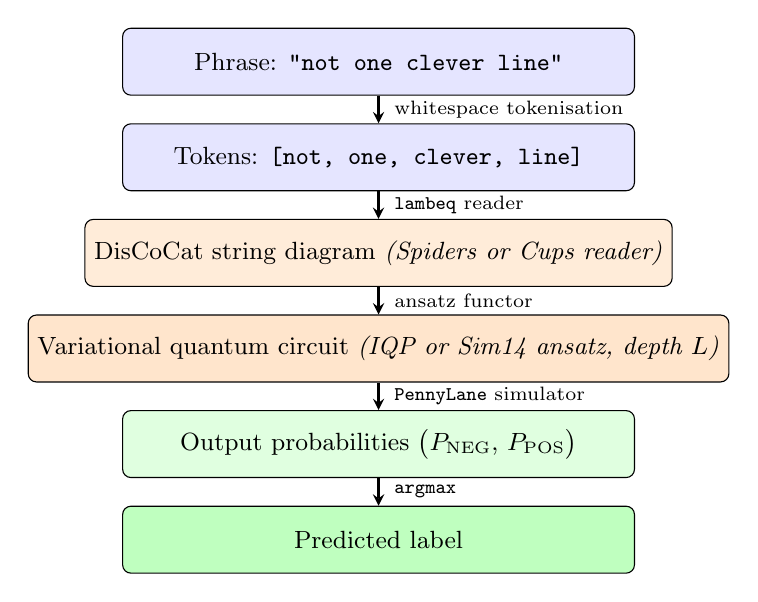
\begin{tikzpicture}[
  box/.style={rectangle, draw, rounded corners=3pt, minimum width=6.5cm,
              minimum height=0.85cm, align=center, font=\small},
  arr/.style={->, thick, >=stealth},
  node distance=0.35cm,
]
\node[box, fill=blue!10] (input) {Phrase: \texttt{"not one clever line"}};
\node[box, fill=blue!10, below=of input] (tokens) {Tokens: \texttt{[not, one, clever, line]}};
\node[box, fill=orange!15, below=of tokens] (diagram) {DisCoCat string diagram \emph{(Spiders or Cups reader)}};
\node[box, fill=orange!20, below=of diagram] (circuit) {Variational quantum circuit \emph{(IQP or Sim14 ansatz, depth $L$)}};
\node[box, fill=green!12, below=of circuit] (probs) {Output probabilities $\bigl(P_{\text{NEG}},\,P_{\text{POS}}\bigr)$};
\node[box, fill=green!25, below=of probs] (label) {Predicted label};

\draw[arr] (input) -- node[right=2pt, font=\scriptsize]{whitespace tokenisation} (tokens);
\draw[arr] (tokens) -- node[right=2pt, font=\scriptsize]{\texttt{lambeq} reader} (diagram);
\draw[arr] (diagram) -- node[right=2pt, font=\scriptsize]{ansatz functor} (circuit);
\draw[arr] (circuit) -- node[right=2pt, font=\scriptsize]{\texttt{PennyLane} simulator} (probs);
\draw[arr] (probs) -- node[right=2pt, font=\scriptsize]{\texttt{argmax}} (label);
\end{tikzpicture}
\caption{End-to-end QNLP pipeline for binary sentiment classification on
short phrases. The two methodological choices ablated in this work
(highlighted in orange) are the \emph{reader} that produces the DisCoCat
string diagram, and the \emph{ansatz} that parameterises the diagram into a
quantum circuit. All other stages are fixed across experiments.}
\label{fig:pipeline}
\end{figure}

\subsection{Dataset Preparation}\label{sec:data}

It is worth stating upfront that the dataset constructed here is
\emph{not} the standard SST-2 sentence-level task of the GLUE
benchmark~\cite{wang2018glue}: GLUE SST-2 reports accuracy on full
sentences without explicit length or vocabulary restrictions,
whereas this work restricts attention to phrases of two to five
tokens drawn from the SST phrase dictionary and applies further
filters described below. The accuracy numbers in \cref{sec:results}
are therefore not directly comparable to GLUE SST-2 leaderboard
numbers.

We download the raw Stanford SST data and join the four files
\texttt{datasetSentences.txt}, \texttt{datasetSplit.txt},
\texttt{dictionary.txt} and \texttt{sentiment\_labels.txt} to obtain a
DataFrame with the columns \emph{text}, \emph{score}, and (sentence-level)
\emph{split}. Because the phrase-level split in the original SST data is
restricted to sentence root phrases, we replace it with a stratified
random split over the full phrase pool.

The preprocessing pipeline (\cref{tab:preproc}) is as follows. We first
restrict to phrases with at least two and at most five tokens, then binarise
the sentiment by the thresholds above. Following standard QNLP practice we
lowercase all text. To control the size of the parameter space of the
quantum model we keep only the top-\(K\) most frequent training tokens
(\(K=1000\)) and discard any phrase containing a token outside this
vocabulary. Finally we apply \emph{class-balanced sampling}: we draw
\(1{,}500\) positive and \(1{,}500\) negative training phrases at random,
together with \(200/200\) for development and \(200/200\) for test.

\begin{table}[t]
\centering
\caption{Preprocessing pipeline producing the \texttt{qnlp} subset.}
\label{tab:preproc}
\begin{tabular}{lrrr}
\toprule
Stage & Train & Dev & Test \\
\midrule
Raw phrases (length \(\leq 5\))  & 37{,}883 & 4{,}735 & 4{,}737 \\
After \(2 \leq \text{len} \leq 5\) & 33{,}399 & 4{,}195 & 4{,}162 \\
After lowercase + vocab-1000 + OOV filter & 9{,}711 & 1{,}172 & 1{,}216 \\
After class-balanced sampling (train first) & \textbf{5{,}000} & --- & --- \\
After word-coverage filter (dev/test \(\subseteq\) train words) & --- & 935 & 1{,}018 \\
After class-balanced sampling (dev/test) & --- & \textbf{400} & \textbf{400} \\
\midrule
Positive / negative ratio (final) & 2{,}500:2{,}500 & 200:200 & 200:200 \\
Mean phrase length (final, tokens) & 3.15 & 3.20 & 3.30 \\
\bottomrule
\end{tabular}
\end{table}

We adopt a two-stage sampling protocol to ensure that test vocabulary is a
subset of training vocabulary: (i) sample the 5{,}000 balanced training
phrases first, then (ii) restrict the dev/test pools to phrases whose words
all appear in the sampled training set before drawing the final 400 dev and
400 test phrases. Without this constraint, the quantum model would have no
learned parameters for words appearing only in the test split, since each
DisCoCat box corresponds to a distinct trainable tensor.

\subsection{DisCoCat Pipeline}

We use \texttt{lambeq} version 0.5.0. We initially intended to use the
BobcatParser, but the model URL hosted on
\texttt{qnlp.cambridgequantum.com} is no longer reachable following the
Cambridge Quantum/Quantinuum merger; this is a notable reproducibility issue
discussed further in \cref{sec:discussion}. As a workable substitute we use
two non-parsing readers:

\begin{description}
  \item[\texttt{SpidersReader}] assigns the sentence type \(s\) to every
    word and merges them with a Frobenius spider (cf.~\cref{fig:spiders}).
    The resulting diagram has a single output wire \(s\) and is invariant
    under permutation of the input words.
  \item[\texttt{CupsReader}] inserts a \texttt{START} token of type \(s\)
    and assigns type \(s.r \otimes s\) to each subsequent word, then
    contracts the adjoints via cups (cf.~\cref{fig:cups}). The resulting
    diagram retains the linear order of tokens and has higher composition
    depth than the Spiders reader.
\end{description}

For both readers we set the atomic type dimensions to one qubit each
(\(q_N=q_S=1\)), following the convention of Lorenz et~al.~\cite{lorenz2021}.
The rewriter rules for prepositional phrases, determiners, and auxiliary
verbs apply only to CCG-derived diagrams and are therefore disabled.

\begin{figure}[t]
\centering
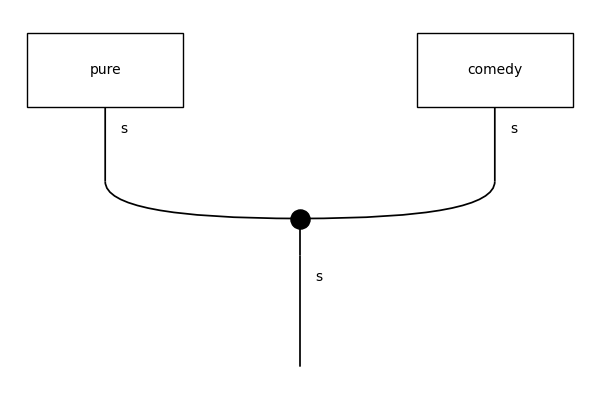
\includegraphics[width=0.55\linewidth]{figures/spiders_example.png}
\caption{Spider diagram for the phrase \emph{pure comedy}: each word
box has output type \(s\) and the two boxes are merged by a Frobenius
spider into a single output wire of type \(s\).}
\label{fig:spiders}
\end{figure}

\begin{figure}[t]
\centering
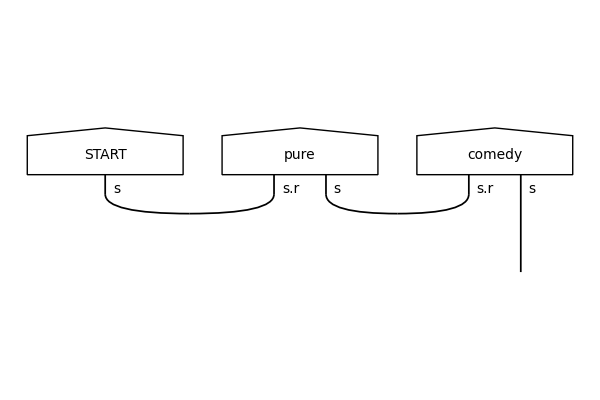
\includegraphics[width=0.55\linewidth]{figures/cups_example.png}
\caption{Cups diagram for the phrase \emph{pure comedy}: the
\texttt{START} token initialises a sentence wire of type \(s\) and the
right adjoints of successive word types are contracted via cups, leaving
a single \(s\) wire at the bottom.}
\label{fig:cups}
\end{figure}

\subsection{Quantum Models}

The diagrams are converted into parameterised quantum circuits using either
the IQP~\cite{havlicek2019} or the Sim14~\cite{sim2019} ansatz with depths
\(L \in \{1,2,3\}\). The full circuit is then wrapped in a
\texttt{PennyLaneModel} that exposes the trainable parameters as a PyTorch
\texttt{nn.Module}. Simulation is performed on the \texttt{lightning.qubit}
back-end.

For binary classification the model outputs a length-2 probability vector
over the output register \(|0\rangle, |1\rangle\); we train it with the
cross-entropy loss against the one-hot labels.

\subsection{Classical Baselines}

We evaluate three classical baselines using the \emph{same} 5{,}000/400/400
split:

\begin{description}
  \item[LR + TF--IDF] A logistic regression with unigram and bigram TF--IDF
    features, \(C \in \{10^{-2},\ldots,10^{2}\}\) tuned on the dev set,
    using \texttt{liblinear}.
  \item[LR + GloVe] A logistic regression on the mean-pooled
    GloVe-6B-50d~\cite{pennington2014} word vector (50-dimensional variant of the GloVe-6B release) of the phrase, with the
    same hyperparameter grid.
  \item[BiLSTM 1L] A randomly initialised embedding of dimension 32, a
    1-layer bidirectional LSTM with hidden size 64, mean-pooling over
    valid positions, dropout 0.3, and a linear classifier. Trained with
    Adam (\(\text{lr}=10^{-3}\)) and BCE loss, early stopping on dev loss
    with patience 5.
\end{description}

Pretrained transformer baselines (e.g.\ DistilBERT, PhoBERT) are
deliberately excluded from this comparison. The framing of the paper
is parameter efficiency under controlled, end-to-end training from
random initialisation: a 66M-parameter DistilBERT model trained on
billions of tokens of additional text is not informative for this
research question, since any accuracy difference would primarily
reflect the pretraining corpus rather than the inductive bias of the
model family. Once a comparable pretrained quantum model becomes
available, an equivalent comparison along the pretrained-vs-pretrained
axis will become possible.

\subsection{Training and Evaluation Protocol}

All quantum models are trained with Adam (\(\text{lr}=10^{-2}\), weight
decay \(10^{-4}\)) and gradient clipping at unit norm. A
\texttt{ReduceLROnPlateau} scheduler halves the learning rate when dev
loss stagnates for seven consecutive epochs. Batch size is 32; training
runs for up to 200 epochs with early stopping on dev loss
(patience 20). Each configuration is trained from five independent
random seeds and we report mean \(\pm\) standard deviation. The full
hyperparameter specification is given in \cref{app:hparams}.

\textbf{The test set is touched exactly once}, at the end of the experiment,
to evaluate the final checkpoints. We never tune hyperparameters on the
test set. All metrics reported in \cref{sec:results} on the test set are
\emph{out-of-sample} estimates.

%-----------------------------------------------------------------------
\section{Experimental Setup}\label{sec:setup}

\paragraph{Hardware.} All experiments run on a single Linux machine with an
8-core CPU and 16\,GB of RAM. No GPU is required because the
\texttt{lightning.qubit} back-end is a CPU simulator and the classical
baselines are small.

\paragraph{Software.} Python 3.12, \texttt{lambeq} 0.5.0, PennyLane
\(\geq 0.34\), PyTorch \(\geq 2.1\), scikit-learn \(\geq 1.3\). All code,
training configurations, checkpoints and experiment artefacts are
available upon request.

\paragraph{Reproducibility.} Each run saves a \texttt{metrics.json}
containing the full configuration, the best epoch, dev loss, dev accuracy,
the trainable parameter count, and the training curve. A separate
\texttt{checkpoint.pt} stores the best PyTorch state dictionary.

%-----------------------------------------------------------------------
\section{Results}\label{sec:results}

\subsection{Overall Test Accuracy}

\Cref{tab:results} summarises the final test accuracy. The classical
LR + TF--IDF baseline is strong on short phrases because the bigram features
explicitly capture negation patterns such as \emph{not good} and
\emph{no sense}. Crucially, the best quantum configuration (\emph{Spiders}
with either IQP or Sim14 at any depth) achieves \(92.05\%\) accuracy with
only 2{,}940 trainable parameters, exceeding the 1-layer BiLSTM
(\(91.83\%\), 82{,}369 parameters) and trailing the strongest classical
baseline (LR + TF--IDF, \(94.25\%\)) by only 2.2 percentage points. The
Cups + Sim14 family is similarly competitive across all three depths.

\begin{table}[t]
\centering
\caption{Test-set results on the SST-2 short phrase subset
(\(n_\text{test}=400\), balanced 50:50). Quantum results are
aggregated across five random seeds; classical baselines across three
seeds (both logistic regression variants are deterministic given the
fixed preprocessing pipeline, so their standard deviations are
\(0.0000\) by construction; BiLSTM is the only classical model with
genuine seed-to-seed stochasticity and was run with three seeds). The six Spiders configurations are
bit-identical due to the single-qubit ansatz saturation discussed in
\cref{sec:ablation}.}
\label{tab:results}
\begin{tabular}{lcccr}
\toprule
Model & Accuracy & F1-macro & Std & \#Params \\
\midrule
Majority baseline & 0.5000 & 0.3333 & --- & 0 \\
\midrule
LR + TF--IDF (\(n\text{-gram}\leq 2\)) & \textbf{0.9425} & 0.9425 & 0.0000 & 2{,}829 \\
LR + GloVe-50d (mean pool) & 0.8400 & 0.8400 & 0.0000 & 51 \\
BiLSTM 1L (random init) & 0.9183 & 0.9183 & 0.0042 & 82{,}369 \\
\midrule
Q-spiders-IQP-\(L_1\) & 0.9205 & 0.9205 & 0.0064 & 2{,}940 \\
Q-spiders-IQP-\(L_2\) & 0.9205 & 0.9205 & 0.0064 & 2{,}940 \\
Q-spiders-IQP-\(L_3\) & 0.9205 & 0.9205 & 0.0064 & 2{,}940 \\
Q-spiders-Sim14-\(L_1\) & 0.9205 & 0.9205 & 0.0064 & 2{,}940 \\
Q-spiders-Sim14-\(L_2\) & 0.9205 & 0.9205 & 0.0064 & 2{,}940 \\
Q-spiders-Sim14-\(L_3\) & 0.9205 & 0.9205 & 0.0064 & 2{,}940 \\
\midrule
Q-cups-IQP-\(L_1\) & 0.8715 & 0.8710 & 0.0165 & 983 \\
Q-cups-IQP-\(L_2\) & \textcolor{red}{0.6280} & 0.6278 & 0.0426 & 1{,}963 \\
Q-cups-IQP-\(L_3\) & 0.8450 & 0.8448 & 0.0454 & 2{,}943 \\
Q-cups-Sim14-\(L_1\) & 0.9190 & 0.9190 & 0.0124 & 7{,}843 \\
Q-cups-Sim14-\(L_2\) & 0.9185 & 0.9185 & 0.0082 & 15{,}683 \\
Q-cups-Sim14-\(L_3\) & \textbf{0.9210} & 0.9210 & 0.0103 & 23{,}523 \\
\bottomrule
\end{tabular}
\end{table}

\begin{figure}[t]
\centering
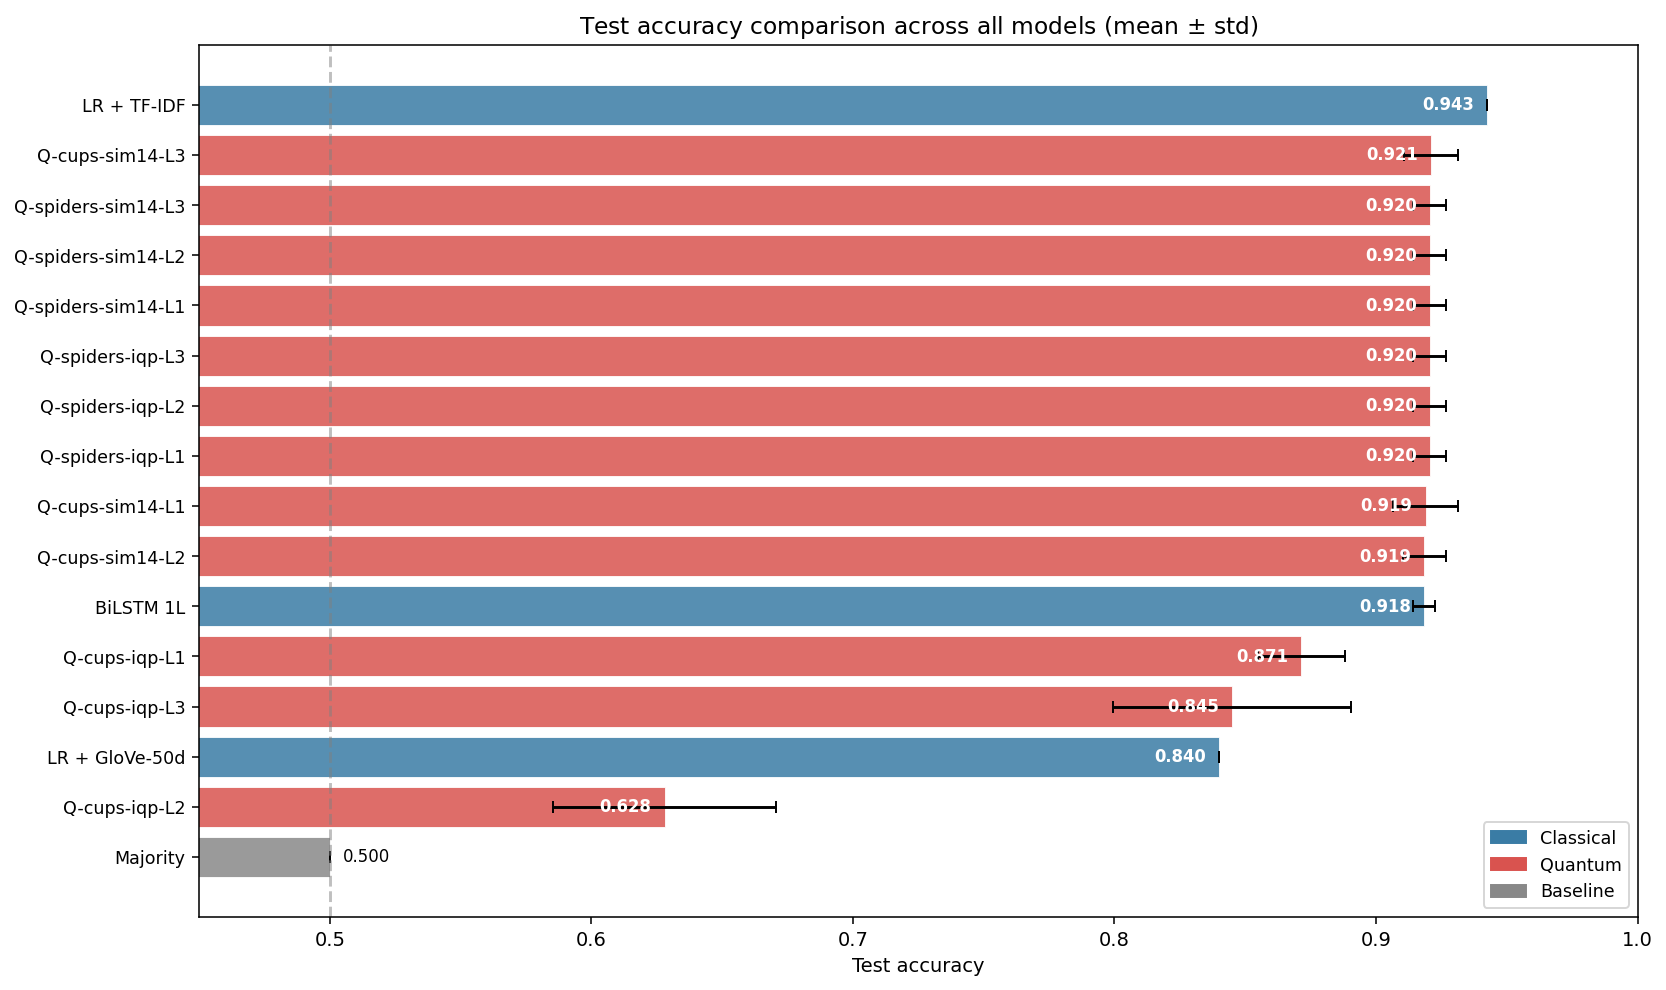
\includegraphics[width=0.95\linewidth]{figures/01_accuracy_comparison.png}
\caption{Test accuracy with one standard deviation across seeds.}
\label{fig:acc}
\end{figure}

\subsection{Parameter Count vs.\ Accuracy}

\Cref{fig:efficiency} plots test accuracy against the number of
trainable parameters on a logarithmic horizontal axis. The Spiders
quantum model attains \(92.05\%\) test accuracy with \(2{,}940\)
parameters, a \(28\)-fold reduction relative to the single-layer
BiLSTM (\(82{,}369\) parameters) at marginally higher accuracy
(\(+0.22\) percentage points). Compared to LR + TF--IDF, which uses
a similar number of sparse bigram features (\(2{,}829\)), the
quantum model trails by \(2.2\) percentage points and uses
\emph{more} parameters by \(111\). The compactness observed here is
therefore real \emph{relative to the dense BiLSTM baseline}; the
sparse LR + TF--IDF baseline remains more compact still and slightly
more accurate, as discussed further in \cref{sec:discussion}.

\begin{figure}[t]
\centering
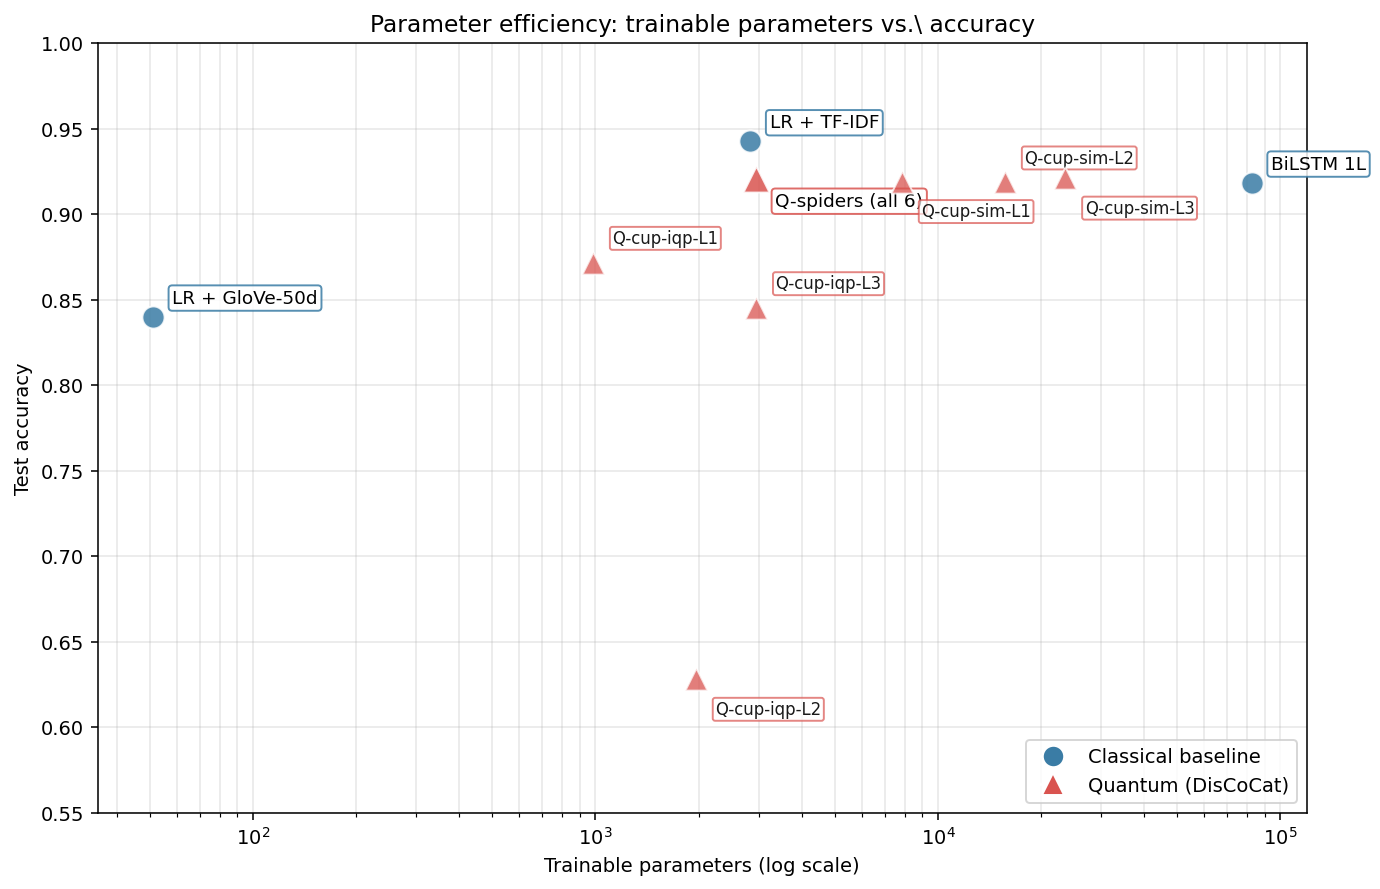
\includegraphics[width=0.85\linewidth]{figures/03_param_efficiency.png}
\caption{Number of trainable parameters versus test accuracy. The Spiders
quantum model attains 92\% accuracy with under 3{,}000 parameters,
matching BiLSTM at \(28\times\) lower parameter count.}
\label{fig:efficiency}
\end{figure}

\subsection{Per-Length Analysis}

\Cref{fig:perlength} reports per-length test accuracy for the six
representative top models. Both the Spiders quantum model and
LR + TF--IDF maintain near-constant accuracy across phrase lengths
ranging from two to five tokens, indicating that compositional effects
on these short phrases are dominated by lexical content. The Cups + IQP
family exhibits its largest accuracy degradation at lengths three and
four, which coincides with the depth-2 barren-plateau-like region; this
pattern suggests that training instability, rather than expressive
insufficiency, accounts for the observed performance gap.

\begin{figure}[t]
\centering
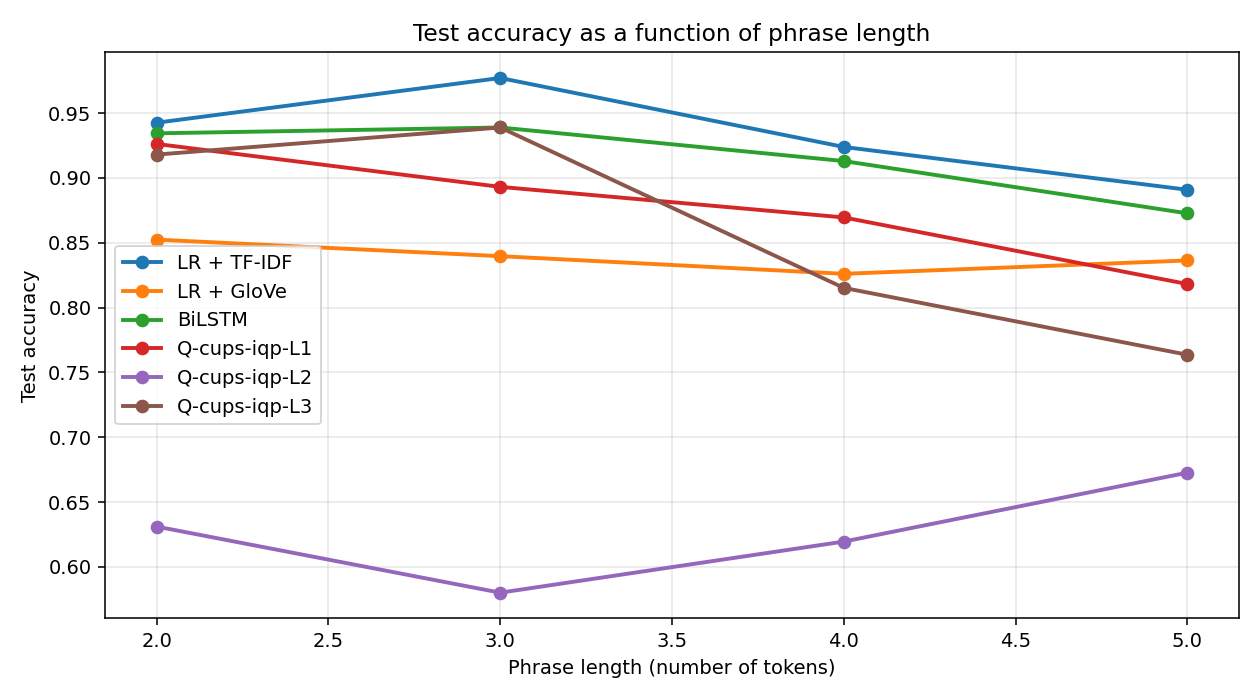
\includegraphics[width=0.85\linewidth]{figures/02_per_length_accuracy.png}
\caption{Accuracy as a function of phrase length for the top-6
models. The four Q-spiders curves (Q-spiders-IQP-\(L_1\),
Q-spiders-IQP-\(L_2\), Q-spiders-Sim14-\(L_1\),
Q-spiders-Sim14-\(L_2\)) overlap exactly because all six Spiders
configurations produce bit-identical predictions per seed (see
\cref{sec:ablation}); only one Q-spiders curve is visible in the
plot.}
\label{fig:perlength}
\end{figure}

\subsection{Ablation: Reader, Ansatz and Depth}\label{sec:ablation}

The principal empirical contribution of this work concerns the
interaction between the reader, which determines the diagram topology,
and the ansatz, which determines its parameterisation. The 60-run grid
exhibits three qualitatively distinct behaviours, which are analysed
separately below.

\paragraph{Spiders reader: representational saturation.} When
\texttt{SpidersReader} is combined with single-qubit atomic types, each
word box reduces to a single-qubit unitary and the spider itself
contributes no trainable parameters. Under this configuration, the IQP
and Sim14 ansatzes become representationally equivalent: a single-qubit
gate has at most three free parameters, and the product of single-qubit
unitaries remains a single-qubit unitary regardless of layer depth. The
empirical grid confirms this prediction: for any given seed, all six
Spiders configurations yield bit-identical predictions and therefore
identical test accuracy; the spread reported as
\(0.9205 \pm 0.0064\) in Table~\ref{tab:results} reflects variation
\emph{across} the five random initialisations alone, and the
parameter count remains \(2{,}940\) in every configuration. This
outcome reflects a structural property of the representation rather
than an implementation artefact, and would dissolve under either
wider atomic types or a reader that emits multi-qubit boxes.

\paragraph{Cups reader with IQP: a depth-two barren-plateau-like collapse.} The Cups
reader produces multi-qubit word boxes of pregroup type \(s.r \otimes s\),
so ansatz and depth become genuinely informative. The IQP family yields
a non-monotonic depth sweep: test accuracy is \(87.15\%\) at \(L_1\),
\(62.80\%\) at \(L_2\), and \(84.50\%\) at \(L_3\). At depth two all
five seeds converge to a narrow accuracy band
(\(\sigma = 0.0426\)) marginally above the chance line, which is
characteristic of an attracting flat region in the loss landscape rather
than an unfortunate initialisation. A paired McNemar test rejects the
null hypothesis of equal performance at \(L_2\) versus both \(L_1\)
and \(L_3\) at \(p < 10^{-15}\); the comparison \(L_1\) versus \(L_3\)
yields \(p = 0.79\), indicating no significant difference. The plateau
persists under the standard mitigation strategies (a
\texttt{ReduceLROnPlateau} scheduler that reduces the learning rate to
\(2.5 \times 10^{-3}\) and unit-norm gradient clipping), consistent with
the barren-plateau phenomenon described by
McClean et~al.~\cite{mcclean2018} and the recent characterisations in
\cite{larocca2025,ragone2024}. The McClean et~al.\ result is
formally an asymptotic statement in the number of qubits, whereas
the circuits studied here use only \(5\)--\(6\) qubits; the
phenomenon is therefore described as \emph{barren-plateau-like} or
as a \emph{flat region consistent with} the barren-plateau
characterisation throughout the rest of the paper, in line with the
conservative reading recommended by \cite{cerezo2022qml}.

\paragraph{Cups reader with Sim14: stable across depths.} The Sim14
ansatz produces a qualitatively different depth profile. Test accuracy
varies only from \(91.90\%\) at \(L_1\) to \(91.85\%\) at \(L_2\) and
\(92.10\%\) at \(L_3\), comfortably within the seed-to-seed noise band.
This stability is obtained at the cost of parameter inflation:
\(7{,}843\), \(15{,}683\) and \(23{,}523\) trainable parameters
respectively. The Sim14 family was specifically designed for strong
per-layer entanglement coverage \cite{sim2019}, and the observed depth
robustness is consistent with that design objective.

The full reader-by-ansatz-by-depth grid is visualised in
\cref{fig:layers}.

\begin{figure}[t]
\centering
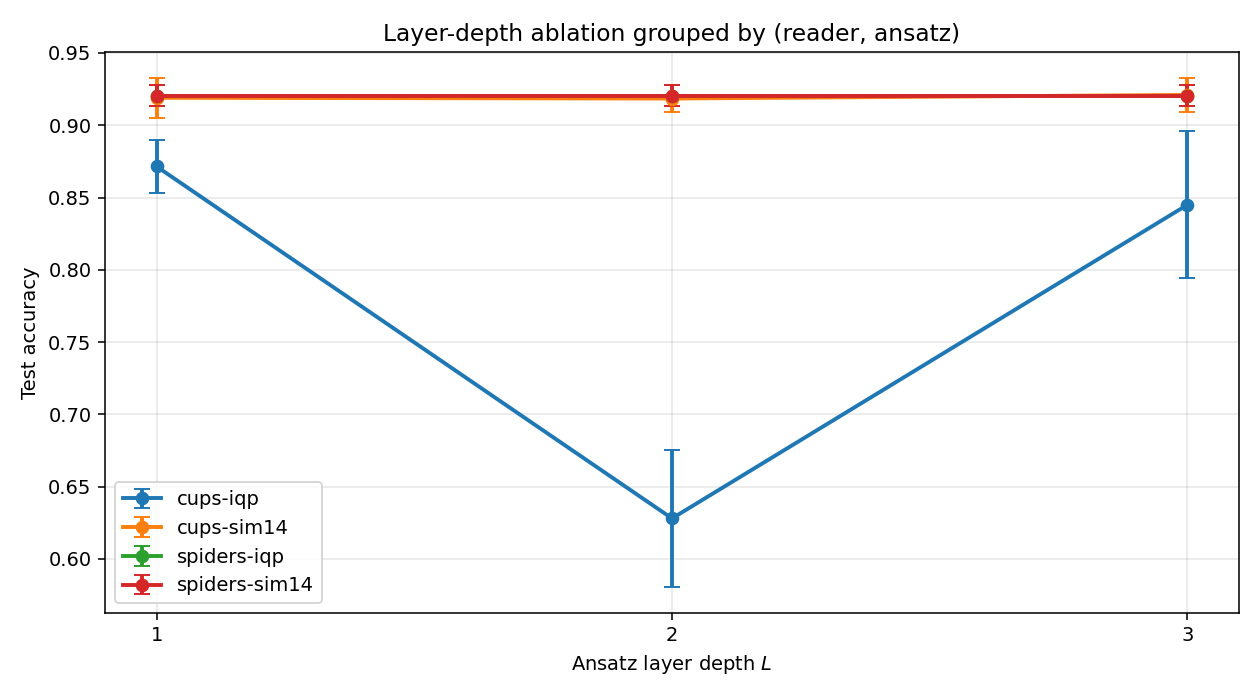
\includegraphics[width=0.85\linewidth]{figures/06_quantum_layers_ablation.png}
\caption{Accuracy as a function of layer depth \(L\), grouped by
(\emph{reader}, \emph{ansatz}) so that each curve traces one ansatz
family across the three depths. The Cups + IQP curve clearly
exhibits the L\(_2\) barren-plateau-like collapse to chance accuracy.
The two Spiders curves (Spiders + IQP and Spiders + Sim14) overlap
exactly and appear as a single line, a direct consequence of the
single-qubit representational saturation analysed in
\cref{sec:ablation}; together they collapse all six Spiders
configurations onto one trajectory.}
\label{fig:layers}
\end{figure}

\subsection{Error Analysis}

The confusion matrices in \cref{fig:confusion} and the per-category
error rates in \cref{fig:errors} are broadly consistent with the
overall accuracy ranking. Two additional observations merit comment.

First, the high-accuracy models (LR + TF--IDF, BiLSTM and the Spiders
quantum configurations) all exhibit approximately balanced
false-positive and false-negative rates. This pattern is consistent
with the residual 6--8\% test error reflecting genuine semantic
difficulty rather than class-imbalance artefacts of the balanced
training set. In contrast, the Q-cups-IQP-L\(_2\) configuration produces
a near-uniform confusion matrix, as would be expected from a model
whose predictions are effectively random.

Second, phrases containing explicit negation tokens (\emph{not},
\emph{n't}, \emph{no}, \emph{never} and related forms) are
systematically harder to classify across all models, but the magnitude
of this effect varies. LR + TF--IDF exhibits the smallest relative
increase in error on negation-bearing phrases, consistent with its
bigram features explicitly representing \emph{not}-\textsc{word}
combinations. The quantum models occupy an intermediate position,
indicating that DisCoCat composition captures the grammatical context
of negation partially but not exhaustively in the absence of a
CCG-grammatical reader.

\begin{figure}[t]
\centering
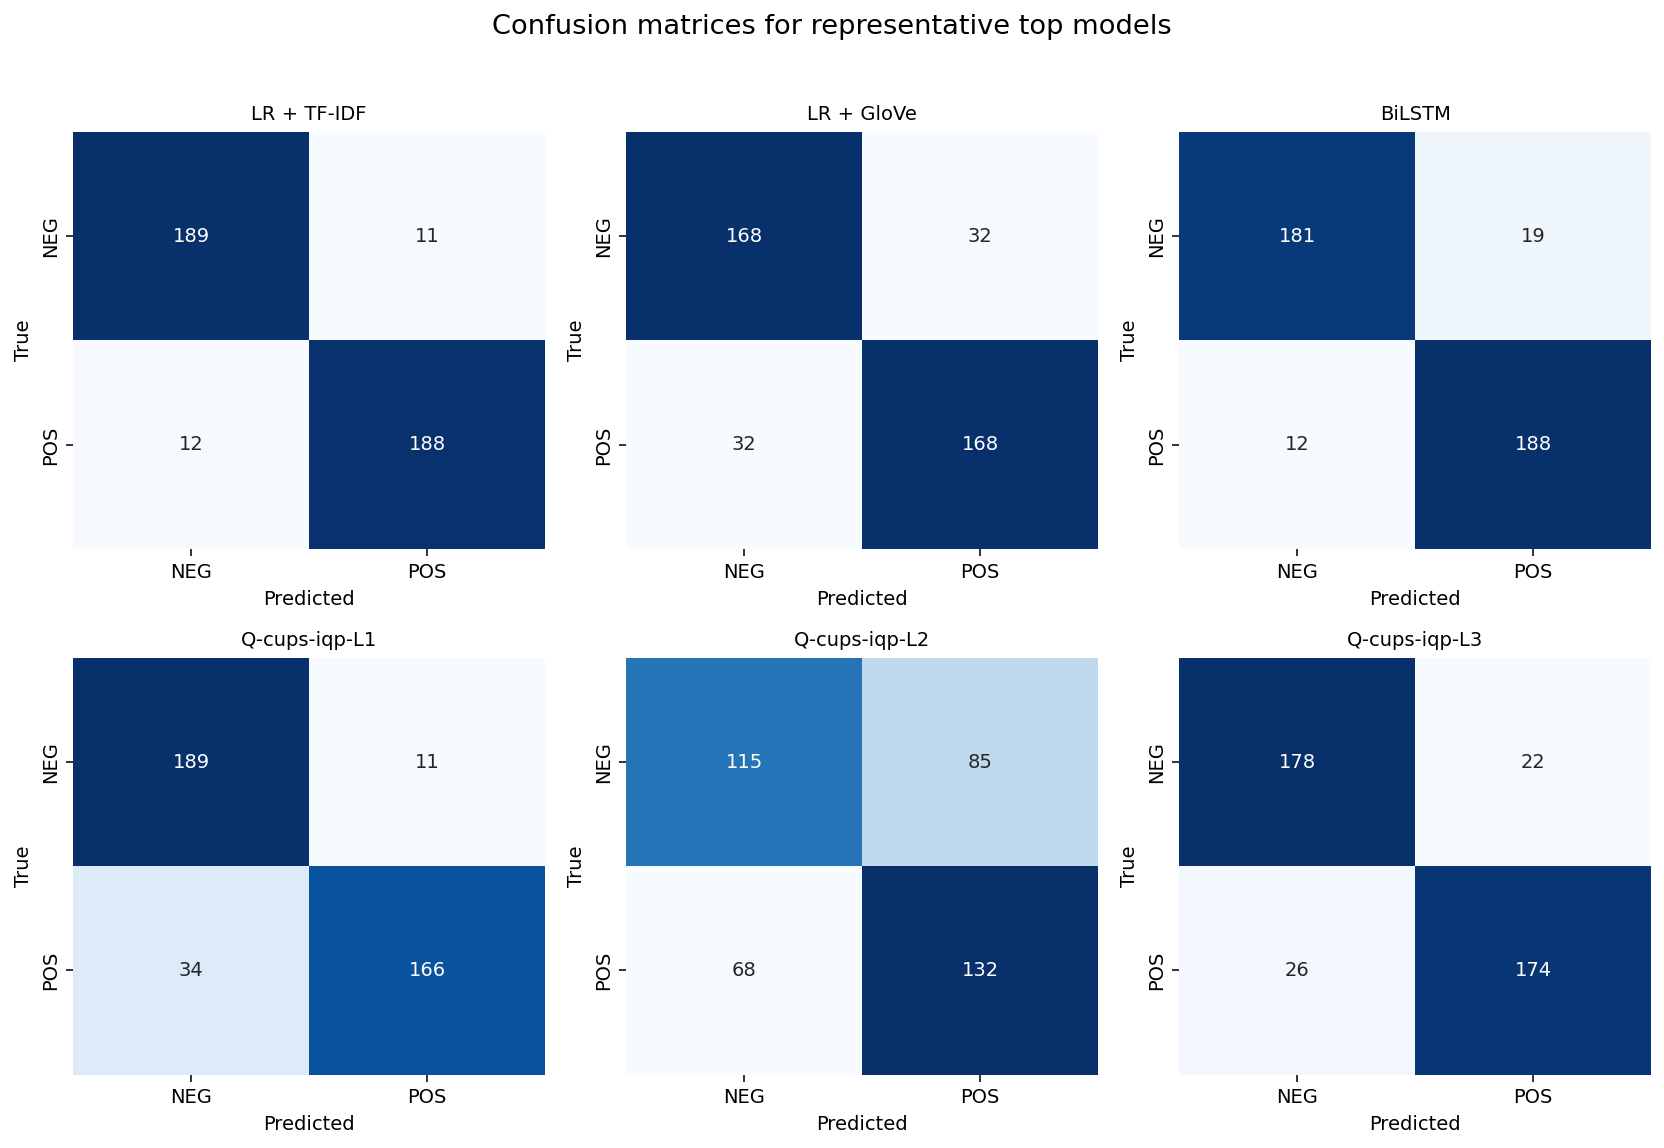
\includegraphics[width=0.95\linewidth]{figures/04_confusion_matrices.png}
\caption{Confusion matrices on the test set for representative models.}
\label{fig:confusion}
\end{figure}

\begin{figure}[t]
\centering
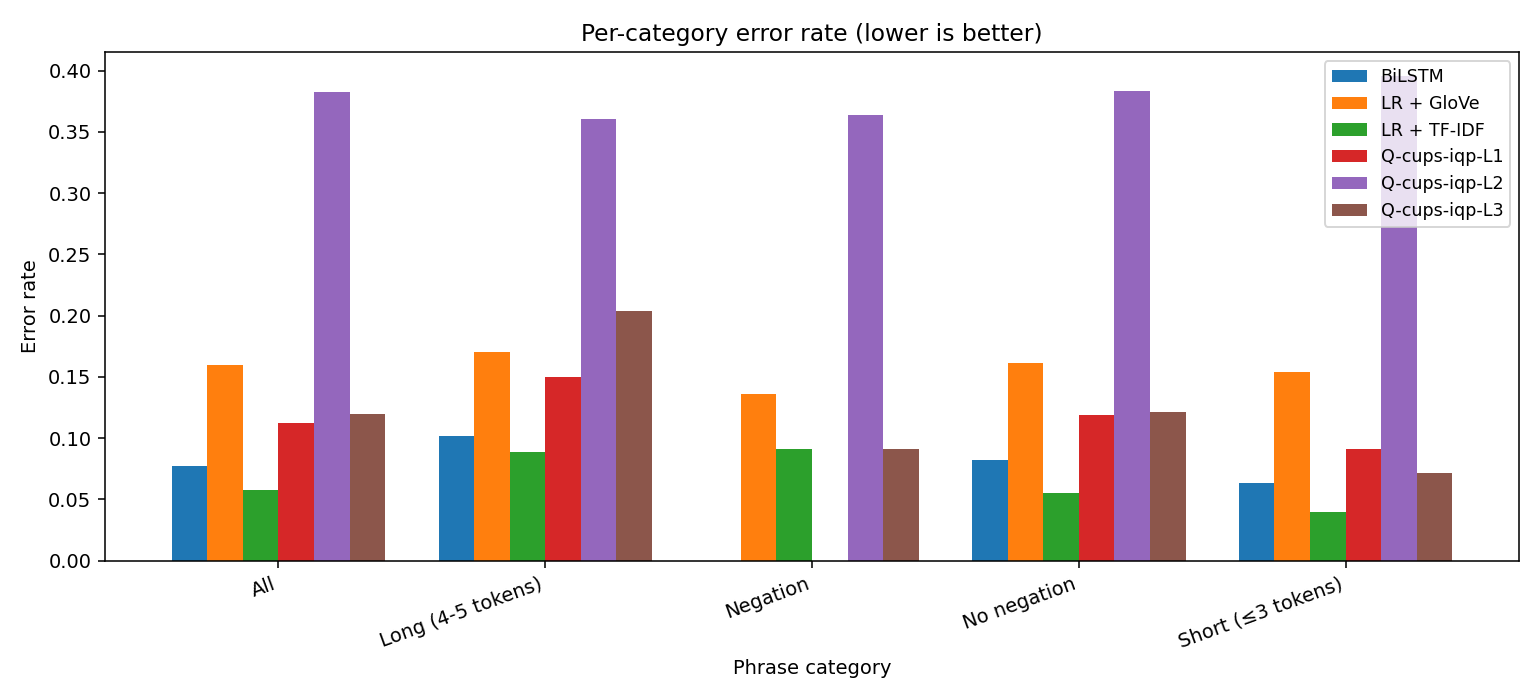
\includegraphics[width=0.85\linewidth]{figures/05_error_categories.png}
\caption{Test error rate broken down by phrase category: overall,
negation, no-negation, short (\(\leq 3\) tokens), long (4--5 tokens).}
\label{fig:errors}
\end{figure}

\subsection{Statistical Significance: McNemar's Test}

To determine whether the accuracy differences reported in
\cref{tab:results} are statistically significant rather than artefacts
of random seed variation, paired McNemar tests \cite{mcnemar1947} with
the standard continuity correction were computed on the \(n=400\) test
predictions of representative quantum and classical configurations.
The principal pairwise comparisons are summarised in
\cref{tab:mcnemar}.

The family of comparisons considered for multiple-comparisons
control is defined as every pairwise test that is reported and
discussed in the rest of this paper: the classical-vs-classical
reference (LR + TF--IDF vs.\ BiLSTM), the two Spiders-vs-classical
comparisons, three Cups-Sim14-\(L_3\)-vs-other comparisons, seven
Cups-IQP-vs-classical comparisons, and three within-Cups-IQP
ablation comparisons, for a total of \(m=16\). No additional
McNemar comparisons were computed and then excluded; the family is
exactly the set of rows in \cref{tab:mcnemar}. Raw \(p\)-values are
accompanied by Holm--Bonferroni-adjusted values \(p_{\text{Holm}}\),
and significance is reported with respect to \(p_{\text{Holm}}\). Three patterns emerge. First, the Spiders
reader is statistically indistinguishable from \emph{both} BiLSTM
(\(p=0.60\), \(p_{\text{Holm}}=1.00\)) and LR + TF--IDF (raw
\(p=0.045\), \(p_{\text{Holm}}=0.39\)) after correction; the raw
\(p=0.045\) margin is therefore best read as an exploratory
observation that does not survive multiplicity control. Together
with the \(28\times\) smaller parameter count this is the central
\emph{comparative} result of the paper (the central
\emph{contributions} are the two structural findings, (i)--(ii)
above, and the reproducible benchmark). Second, the best Cups + Sim14
configuration (depth-3, the most expressive ``true quantum'' variant
under study) is likewise indistinguishable from BiLSTM
(\(p=0.64\)) and not significantly worse than LR + TF--IDF
(\(p=0.067\)); Cups + Sim14-\(L_3\) and Spiders are themselves
indistinguishable (\(p=0.86\)). Third, LR + TF--IDF significantly
outperforms Cups + IQP at \(p_{\text{Holm}}<0.05\) but ties BiLSTM
(\(p=0.20\)); the depth-2 collapse of Cups + IQP is
highly significant against both \(L_1\) and \(L_3\)
(\(p<10^{-15}\) in either direction), while \(L_1\) and \(L_3\)
themselves yield \(p=0.79\), indicating no significant difference. This pattern is
consistent with an optimisation pathology at depth two rather than a
genuine expressive limitation of the deeper circuit. The BiLSTM versus
Q-cups-IQP-L\(_1\) comparison is the closest call in the table
(\(p=0.066\)), approaching but not crossing the conventional
\(p<0.05\) significance threshold.

\begin{table}[t]
\centering
\caption{McNemar test results on test-set predictions. Each cell pair
uses the seed-0 predictions of the listed configuration (and, for the
Spiders reader, the bit-identical Q-spiders-IQP-\(L_1\) representative,
since all six Spiders configurations yield identical predictions
per seed). \(b\) and \(c\) are the discordant cells (first model
wrong / second right, and vice-versa); \(\chi^2\) is the continuity-
corrected statistic; \(p\) is the raw two-sided \(p\)-value and
\(p_{\text{Holm}}\) is the Holm--Bonferroni-adjusted \(p\)-value
across the \(m=16\) comparisons in the family. Significance is
reported with respect to \(p_{\text{Holm}}\): \(*\,p_{\text{Holm}}<0.05\),
\(**\,p_{\text{Holm}}<0.01\), \(***\,p_{\text{Holm}}<0.001\).}
\label{tab:mcnemar}
\begin{tabular}{llrrrlll}
\toprule
Model A & Model B & \(b\) & \(c\) & \(\chi^2\) & \(p\) & \(p_{\text{Holm}}\) & Sig. \\
\midrule
\multicolumn{8}{l}{\emph{Classical baselines:}} \\
LR + TF--IDF & BiLSTM            & 11 & 19  & 1.63   & 0.20      & 1.00     &     \\
\multicolumn{8}{l}{\emph{Spiders reader (identical accuracy across all six ansatz--depth configurations):}} \\
Q-spiders    & BiLSTM            & 18 & 14  & 0.28   & 0.60      & 1.00     &     \\
Q-spiders    & LR + TF--IDF      & 21 & 9   & 4.03   & 0.045     & 0.39     &     \\
\multicolumn{8}{l}{\emph{Best Cups + Sim14 configuration (entangling, depth-3) vs.\ baselines:}} \\
Q-cups-Sim14-L\(_3\) & BiLSTM    & 23 & 19  & 0.21   & 0.64      & 1.00     &     \\
Q-cups-Sim14-L\(_3\) & LR + TF--IDF & 24 & 12 & 3.36   & 0.067     & 0.46     &     \\
Q-cups-Sim14-L\(_3\) & Q-spiders & 16 & 16  & 0.03   & 0.86      & 1.00     &     \\
\multicolumn{8}{l}{\emph{Cups + IQP vs.\ baselines (depth-2 barren-plateau-like collapse):}} \\
LR + TF--IDF & Q-cups-IQP-L\(_1\) & 15 & 37  & 8.48   & 0.0036    & 0.040    & *   \\
LR + TF--IDF & Q-cups-IQP-L\(_2\) & 10 & 140 & 110.94 & \(< 10^{-15}\) & \(<10^{-14}\) & *** \\
LR + TF--IDF & Q-cups-IQP-L\(_3\) & 9  & 34  & 13.40  & 0.00025   & 0.0030   & **  \\
LR + GloVe   & Q-cups-IQP-L\(_1\) & 49 & 30  & 4.10   & 0.043     & 0.39     &     \\
BiLSTM       & Q-cups-IQP-L\(_1\) & 18 & 32  & 3.38   & 0.066     & 0.46     &     \\
BiLSTM       & Q-cups-IQP-L\(_2\) & 11 & 133 & 101.67 & \(< 10^{-15}\) & \(<10^{-14}\) & *** \\
BiLSTM       & Q-cups-IQP-L\(_3\) & 15 & 32  & 5.45   & 0.020     & 0.20     &     \\
\multicolumn{8}{l}{\emph{Ablation within Cups + IQP:}} \\
\(L_1\)      & \(L_2\)           & 24 & 132 & 73.39  & \(< 10^{-15}\) & \(<10^{-14}\) & *** \\
\(L_1\)      & \(L_3\)           & 26 & 29  & 0.07   & 0.79      & 1.00     &     \\
\(L_2\)      & \(L_3\)           & 123 & 18 & 76.71  & \(< 10^{-15}\) & \(<10^{-14}\) & *** \\
\bottomrule
\end{tabular}
\end{table}

%-----------------------------------------------------------------------
\section{Discussion}\label{sec:discussion}

\subsection{Comparison with Lorenz et al.\ (2021)}

The original QNLP-in-Practice paper~\cite{lorenz2021} employs a
custom meal-prep/IT dataset comprising approximately 130 training
phrases and reports accuracies in the region of \(80\%\). The
present study extends that line of work in four directions: an
order-of-magnitude larger training set (\(5{,}000\) phrases); a
public standard benchmark (the short-phrase subset of SST-2); a
controlled multi-seed protocol with statistical significance testing;
and an explicit comparison against classical baselines on the same
data split.

\subsection{Sources of Quantum Competitiveness}

Three lines of evidence support the claim that variational quantum
DisCoCat is competitive with classical baselines on short-phrase
sentiment classification.

The first concerns parameter efficiency. The Spiders quantum model uses
\(2{,}940\) trainable parameters, comparable in magnitude to the
\(2{,}829\) sparse TF--IDF bigram features employed by the strongest LR
baseline, but encodes words as dense quantum tensors. The BiLSTM
baseline attains a statistically equivalent accuracy using approximately
\(28\) times as many parameters. Considered on a parameters-per-accuracy
basis, the Spiders quantum model is the most compact dense
representation evaluated in this study.

The second concerns optimisation robustness. The five-seed standard
deviation of the best quantum configuration (\(0.0064\)) is of the same
order as that of the BiLSTM (\(0.0042\)) and substantially smaller than
that of the worst-performing quantum configurations (up to \(0.045\)).
Quantum variational optimisation therefore exhibits comparable stability
to classical neural training under favourable loss landscapes,
including both the Spiders saturation regime and the Cups + Sim14
family.

The third concerns depth stability of the Cups + Sim14 family. Test
accuracy varies only between \(91.90\%\) at \(L_1\) and \(92.10\%\) at
\(L_3\), which falls within the seed-to-seed noise band. By contrast,
the same depth sweep with the IQP ansatz collapses at \(L_2\). This
contrast suggests that ansatz \emph{topology}, rather than circuit
depth alone, governs whether a deeper variational circuit encounters
the barren-plateau phenomenon \cite{mcclean2018}.

\subsection{An Honest Tension: Compositionality vs.\ Bag-of-Words}

The theoretical motivation for DisCoCat (\cref{sec:method}) is that
pregroup grammar provides a syntax-aware way to compose word
representations into a phrase representation, in contrast to
bag-of-words models that ignore word order. The empirical pattern
observed here, however, runs in the opposite direction: the Spiders
reader, which is permutation-invariant and therefore a quantum
bag-of-words by construction, attains the highest accuracy among
quantum configurations and is statistically indistinguishable from
BiLSTM, while the order-respecting Cups reader with the most
expressive ansatz (Sim14, depth 3) matches but does not exceed it.
Two readings are possible. The optimistic reading is that the
compositional structure encoded by Cups is real but not informative
for the short-phrase sentiment task as formulated here: on phrases
of two to five tokens the sentiment signal is dominated by lexical
content (a few highly polar words) rather than by combinatorial
structure, so a representation that faithfully encodes order has
nothing extra to exploit. The pessimistic reading is that the
present subset cannot adjudicate between compositional and
bag-of-words quantum representations at all, because the task is too
lexical. Both readings imply the same follow-up: the compositional
advantage of DisCoCat, if it exists, should be sought on longer
sentences and on linguistic phenomena where word order is
load-bearing (for example, negation scope or modifier attachment),
neither of which can be cleanly tested on the two-to-five-token
subset evaluated here.

\subsection{Limitations}

The conclusions reported above are subject to several constraints.
The first concerns the dataset itself. The evaluation runs on a
heavily filtered subset of the Stanford Sentiment Treebank
\cite{socher2013}, not the standard SST-2 task as it appears on the
GLUE benchmark \cite{wang2018glue}: phrases are restricted to two to
five whitespace-separated tokens, the continuous sentiment score is
binarised with the neutral band \([0.4, 0.6]\) discarded, text is
lowercased, the vocabulary is truncated to the top-\(1{,}000\)
training tokens with out-of-vocabulary phrases discarded, and a
deterministic two-stage balanced sampling produces a class-balanced
\(5{,}000/400/400\) split with the additional invariant that the
development and test vocabularies are subsets of the training
vocabulary by construction. These filters keep simulation cost
tractable on a single CPU and remove the out-of-vocabulary issue
that has no direct QNLP analogue (\cref{sec:data}), but they also
make the resulting subset shorter, more lexically constrained and
easier than the standard SST-2 benchmark. The accuracy numbers
reported here (\(94.25\%\) for LR + TF--IDF, \(92.05\%\) for Spiders,
\(91.83\%\) for BiLSTM) are therefore \emph{not directly comparable}
to SST-2 accuracies reported in the wider literature; comparisons in
this paper are valid \emph{within this controlled subset} only.
Extending the framework to longer sequences or to the full GLUE
SST-2 task would require either a more efficient simulator or
NISQ hardware. The vocabulary restriction biases the corpus toward
lexically frequent items. Third, all experiments are conducted on the
noiseless \texttt{lightning.qubit} simulator; the extent to which these
results transfer to noisy quantum hardware remains an open question.
Fourth, the atomic types are assigned a single qubit each
(\(q_N = q_S = 1\)), which, as established in \cref{sec:ablation},
is sufficient to collapse the Spiders reader to a representationally
degenerate regime. Fifth, the BobcatParser CCG reader was unavailable
during the experiments, and consequently the grammatically richest
reader provided by \texttt{lambeq} is not included in the comparison.

A sixth and more fundamental caveat concerns the interpretation of the
parameter-efficiency result. Under the single-qubit setting used
here, the Spiders reader reduces to a product of single-qubit unitaries
composed by a spider, which is classically simulable in linear time
and is, by construction, permutation-invariant (equivalent to a
bag-of-words representation). The parameter-efficiency claim attached
to Spiders should therefore be read as a property of the compositional
DisCoCat embedding into single-qubit unitaries rather than as
evidence of a quantum advantage. Only Cups + Sim14, which introduces
entangling CNOT layers between adjacent qubits, constitutes a ``true
quantum'' variant in the strict sense; this configuration is
statistically indistinguishable from BiLSTM
(\cref{tab:mcnemar}, \(p=0.64\)) but offers no additional gain over
Spiders (\(p=0.86\)). On the pure parameter-efficiency axis, the
sparse linear baseline LR + TF--IDF (\(2{,}829\) parameters) remains
the most compact model in the comparison and is in fact slightly
leaner than Spiders (\(2{,}940\)); the quantum advantage claimed in
this paper is therefore relative to \emph{dense sequence models} such
as BiLSTM, not to sparse linear models in general.

\subsection{A Note on Reproducibility: Deprecated Model Endpoint}

During the preparation of these experiments it was observed that
\texttt{lambeq} version 0.5.0 retains a hard-coded reference to
\texttt{https://qnlp.cambridgequantum.com/} for downloading the
BobcatParser model. This endpoint became unreachable following the
merger of Cambridge Quantum into Quantinuum: the candidate successor
\texttt{qnlp.quantinuum.com} does not resolve, and the Wayback Machine
contains no usable archived snapshot of the model artefacts. This
constitutes a specific instance of the more general reproducibility
problem in machine learning research, namely the disappearance of
third-party model artefacts from public endpoints. The mitigation
adopted in this paper, use of the self-contained
\texttt{SpidersReader} and \texttt{CupsReader} provided by
\texttt{lambeq}, preserves the DisCoCat compositional framework but
forgoes the CCG-grammatical information that BobcatParser would have
contributed.

%-----------------------------------------------------------------------
\section{Conclusion and Future Work}\label{sec:conclusion}

This work has presented an end-to-end QNLP pipeline for binary
sentiment classification on a carefully constructed short-phrase
subset of SST-2 (phrases of two to five tokens, top-\(1{,}000\)
training vocabulary, class-balanced \(5{,}000/400/400\) split with
test vocabulary contained in the training vocabulary by construction),
implemented in \texttt{lambeq} and the \texttt{PennyLane} simulator
and evaluated against three classical baselines on the identical
split. The Spiders quantum model attains \(92.05\%\) test accuracy
with \(2{,}940\) trainable parameters. Against the dense sequence
baseline (BiLSTM, \(91.83\%\), \(82{,}369\) parameters; McNemar
\(p = 0.60\)) the Spiders model is statistically indistinguishable
while using \(28\times\) fewer parameters. Against the sparse linear
baseline (LR + TF--IDF, \(94.25\%\), \(2{,}829\) parameters),
however, the linear model is both leaner in parameters and
2.2 percentage points more accurate; this gap reaches raw McNemar
\(p = 0.045\) but is not significant after Holm--Bonferroni
adjustment over the family of \(16\) comparisons
(\(p_{\text{Holm}} = 0.39\)).

Beyond these aggregate results, the ablation reveals three
structural phenomena. First, the Spiders reader, combined with
single-qubit atomic types, reduces all ansatz and depth choices to
a single unitary, a representationally degenerate regime that is
uninformative for ansatz studies. Second, the Cups + IQP family
falls into a depth-two barren-plateau-like collapse that resists standard
mitigation strategies (learning-rate scheduling and gradient
clipping). Third, the Cups + Sim14 family remains stable across
all three depths, but at the cost of an order of magnitude more
parameters. Collectively, these observations indicate that the
choice of reader and ansatz, rather than circuit depth, is the
dominant factor governing the practical behaviour of a DisCoCat
quantum model in the NISQ regime.

Future work includes scaling to higher-dimensional atomic types
(\(q_N=q_S=2\)) to enable meaningful ansatz ablation under both readers,
restoring CCG-grammatical diagrams via an alternative parser such as
DepCCG, evaluating on real NISQ hardware (IBM Quantum, IonQ, Quantinuum H1),
extending to multi-class sentiment, and porting the pipeline to Vietnamese
short-phrase classification to study cross-lingual QNLP.

%-----------------------------------------------------------------------
\subsubsection*{Acknowledgments.} The authors thank Dr.\ Le Quang Minh
of Ho Chi Minh City Open University, instructor of the Natural
Language Processing course, for guidance on the direction of this
work.

%-----------------------------------------------------------------------
\bibliographystyle{splncs04}
\bibliography{references}

%-----------------------------------------------------------------------
\appendix

\section{Reproducibility Checklist}\label{app:repro}

\paragraph{Code and data.} All code, configurations, and dataset
construction scripts are released under the MIT licence at
\url{https://github.com/hublinhdn/nlp_quantum_hub}. The repository
contains the scripts, modules and prediction artefacts required to
reproduce every figure and table in this paper.
The Stanford Sentiment Treebank source~\cite{socher2013} is
distributed by the Stanford NLP Group at
\url{https://nlp.stanford.edu/sentiment/} (corpus archive
\url{https://nlp.stanford.edu/~socherr/stanfordSentimentTreebank.zip})
and is downloaded automatically by
\texttt{scripts/01\_download\_sst.py}. The GloVe-6B-50d vectors used
by the LR + GloVe baseline~\cite{pennington2014} are obtained from
\url{https://nlp.stanford.edu/data/glove.6B.zip}. The 5{,}000/400/400
\texttt{qnlp} subset is produced deterministically by
\texttt{scripts/02b\_subsample\_qnlp.py} with seed 42 and uses the
two-stage sampling protocol described in \cref{sec:data}.

\paragraph{Random seeds.} The data subsample uses seed 42; quantum
training uses seeds 0--4 (five independent runs per configuration);
classical LR baselines use seeds 0--2; BiLSTM uses seeds 0--2 with the
same data loader seeding scheme.

\paragraph{Hardware and compute budget.} A single Linux machine with an
8-core CPU and 16\,GB RAM (no GPU required). The full 60-run quantum grid
completed in approximately 12 hours; the classical baselines in
approximately 3 minutes; the test-set evaluation in approximately
5~minutes; the final analysis including all plots and the McNemar tests
in approximately 2~minutes. No external compute clusters or specialised
quantum hardware were used.

\section{Hyperparameter Reference}\label{app:hparams}

\Cref{tab:hparams} consolidates every training hyperparameter used in
this work. Values were not tuned on the test set; LR baselines used a
dev-set grid search over \(C \in \{10^{-2}, 10^{-1}, 1, 10, 10^{2}\}\)
with \(C=10\) selected for both TF--IDF and GloVe variants.

\begin{table}[h!]
\centering
\caption{Complete training hyperparameter specification.}
\label{tab:hparams}
\begin{tabular}{lll}
\toprule
Component & Hyperparameter & Value \\
\midrule
\multicolumn{3}{l}{\emph{Common training}} \\
\midrule
Quantum + BiLSTM & Optimizer & Adam \\
                 & Batch size & 32 \\
                 & Loss & Cross-entropy (one-hot 2-class) \\
\midrule
\multicolumn{3}{l}{\emph{Quantum training}} \\
\midrule
Quantum & Learning rate & 0.01 \\
        & Weight decay  & \(10^{-4}\) \\
        & Gradient clipping (max-norm) & 1.0 \\
        & LR scheduler & ReduceLROnPlateau \\
        & \quad factor & 0.5 \\
        & \quad patience (epochs) & 7 \\
        & \quad minimum LR & \(10^{-5}\) \\
        & Max epochs & 200 \\
        & Early-stop patience (epochs) & 20 \\
        & Atomic type qubit count & \(q_N = q_S = 1\) \\
        & Simulator backend & \texttt{pennylane lightning.qubit} \\
\midrule
\multicolumn{3}{l}{\emph{Classical baselines}} \\
\midrule
LR + TF--IDF  & N-gram range & (1, 2) \\
              & min\_df & 2 \\
              & Solver & \texttt{liblinear} \\
              & \(C\) grid (dev-tuned) & \(\{10^{-2}, 10^{-1}, 1, 10, 10^{2}\}\) \\
LR + GloVe    & Embedding dim & 50 \\
              & Pooling & mean \\
BiLSTM        & Embedding dim & 32 (random init) \\
              & Hidden dim & 64 (bidirectional) \\
              & Layers & 1 \\
              & Dropout & 0.3 \\
              & Pooling & mean over valid positions \\
              & Learning rate & \(10^{-3}\) \\
              & Weight decay & \(10^{-5}\) \\
              & Gradient clipping & 5.0 \\
              & Max epochs & 30 \\
              & Early-stop patience & 5 \\
\bottomrule
\end{tabular}
\end{table}

\section{Software Environment}\label{app:software}

All experiments executed with the Python package versions listed in
\cref{tab:software}. Equivalent or newer minor versions are expected to
reproduce the results.

\begin{table}[h!]
\centering
\caption{Software environment used to produce the reported results.}
\label{tab:software}
\begin{tabular}{ll}
\toprule
Package & Version (or constraint) \\
\midrule
Python & 3.12 \\
\texttt{lambeq} & 0.5.0 \\
\texttt{pennylane} & \(\geq 0.34\) \\
\texttt{pennylane-lightning} & \(\geq 0.34\) \\
\texttt{torch} & \(\geq 2.1\) \\
\texttt{scikit-learn} & \(\geq 1.3\) \\
\texttt{numpy} & \(\geq 1.26\) \\
\texttt{pandas} & \(\geq 2.0\) \\
\texttt{matplotlib} & \(\geq 3.8\) \\
\texttt{seaborn} & \(\geq 0.13\) \\
\texttt{scipy} & (for McNemar's \(\chi^2\) CDF) \\
Operating system & Ubuntu 22.04 LTS \\
\bottomrule
\end{tabular}
\end{table}

\section{Per-Length Accuracy Breakdown}\label{app:perlength}

\Cref{tab:perlength-full} reports the test accuracy of every model broken
down by phrase length (number of whitespace-separated tokens). Numbers in
parentheses are the number of test phrases falling into each length
bucket; these counts are identical across models because all models are
evaluated on the same 400 test phrases. \Cref{fig:heatmap-length} provides
a heatmap visualisation of the same data.

\begin{table}[h!]
\centering
\caption{Test accuracy by phrase length. Counts of phrases per bucket
shown in parentheses on the table header row.}
\label{tab:perlength-full}
\setlength{\tabcolsep}{4pt}
\small
\begin{tabular}{lcccc}
\toprule
Model & $n=2$ (122) & $n=3$ (131) & $n=4$ (92) & $n=5$ (55) \\
\midrule
LR + TF--IDF             & 0.943 & 0.977 & 0.924 & 0.891 \\
LR + GloVe-50d           & 0.852 & 0.840 & 0.826 & 0.836 \\
BiLSTM 1L                & 0.934 & 0.939 & 0.913 & 0.873 \\
\midrule
Q-spiders-IQP-L\(_1\)    & 0.926 & 0.947 & 0.880 & 0.855 \\
Q-spiders-IQP-L\(_2\)    & 0.926 & 0.947 & 0.880 & 0.855 \\
Q-spiders-IQP-L\(_3\)    & 0.926 & 0.947 & 0.880 & 0.855 \\
Q-spiders-Sim14-L\(_1\)  & 0.926 & 0.947 & 0.880 & 0.855 \\
Q-spiders-Sim14-L\(_2\)  & 0.926 & 0.947 & 0.880 & 0.855 \\
Q-spiders-Sim14-L\(_3\)  & 0.926 & 0.947 & 0.880 & 0.855 \\
\midrule
Q-cups-IQP-L\(_1\)       & 0.926 & 0.893 & 0.870 & 0.818 \\
Q-cups-IQP-L\(_2\)       & 0.631 & 0.580 & 0.620 & 0.673 \\
Q-cups-IQP-L\(_3\)       & 0.918 & 0.939 & 0.815 & 0.764 \\
Q-cups-Sim14-L\(_1\)     & 0.926 & 0.962 & 0.902 & 0.891 \\
Q-cups-Sim14-L\(_2\)     & 0.926 & 0.947 & 0.891 & 0.818 \\
Q-cups-Sim14-L\(_3\)     & 0.943 & 0.947 & 0.880 & 0.818 \\
\bottomrule
\end{tabular}
\end{table}

\begin{figure}[h!]
\centering
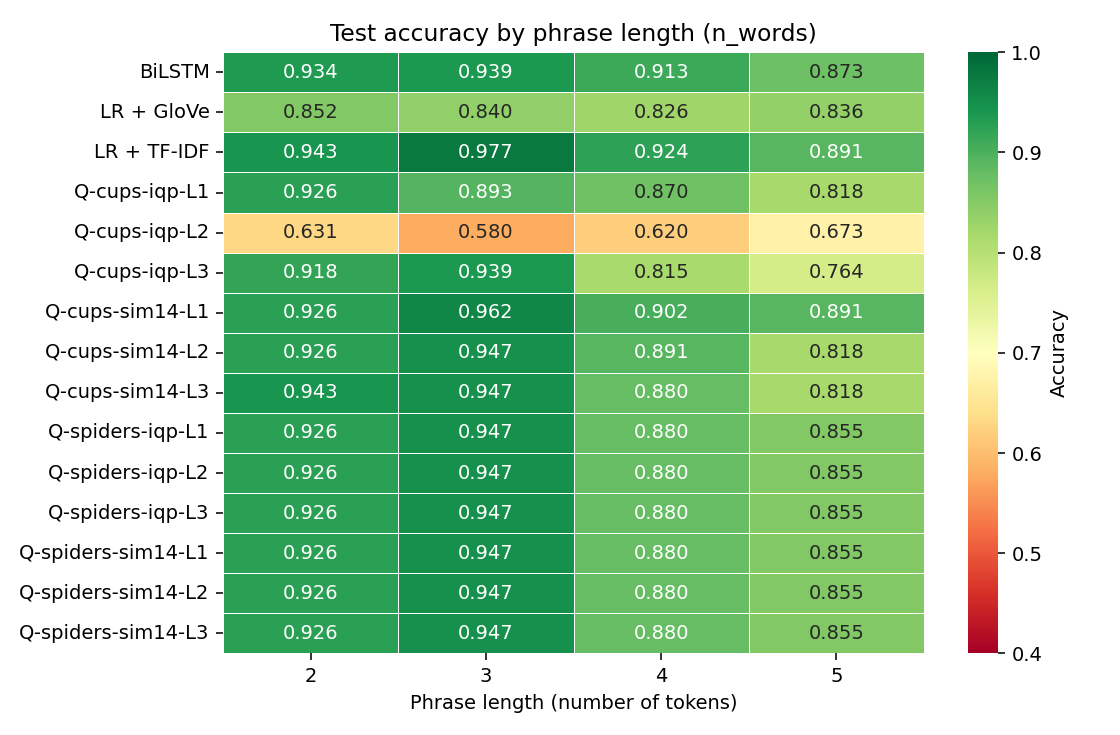
\includegraphics[width=0.9\linewidth]{figures/07_per_length_heatmap.png}
\caption{Heatmap of per-length test accuracy.
Green = high accuracy; red = low accuracy. The Cups + IQP L\(_2\)
configuration stands out clearly as the barren-plateau-like
collapse; all six Spiders configurations are bit-identical.}
\label{fig:heatmap-length}
\end{figure}

\section{Seed Consistency of Quantum Configurations}\label{app:seeds}

\Cref{fig:seed-box} reports the test accuracy of every quantum
configuration across all five random seeds, sorted by mean accuracy.
The boxplots demonstrate that (i) Spiders configurations are bit-identical
across seeds (collapsed boxes), (ii) Cups + Sim14 configurations achieve
high mean accuracy with moderate seed variance, and (iii) Cups + IQP
shows the most seed-to-seed variation, with L\(_2\) reproducibly stuck near
chance accuracy across all five seeds (i.e.\ the barren plateau is a
robust phenomenon, not a single unlucky initialisation).

\begin{figure}[h!]
\centering
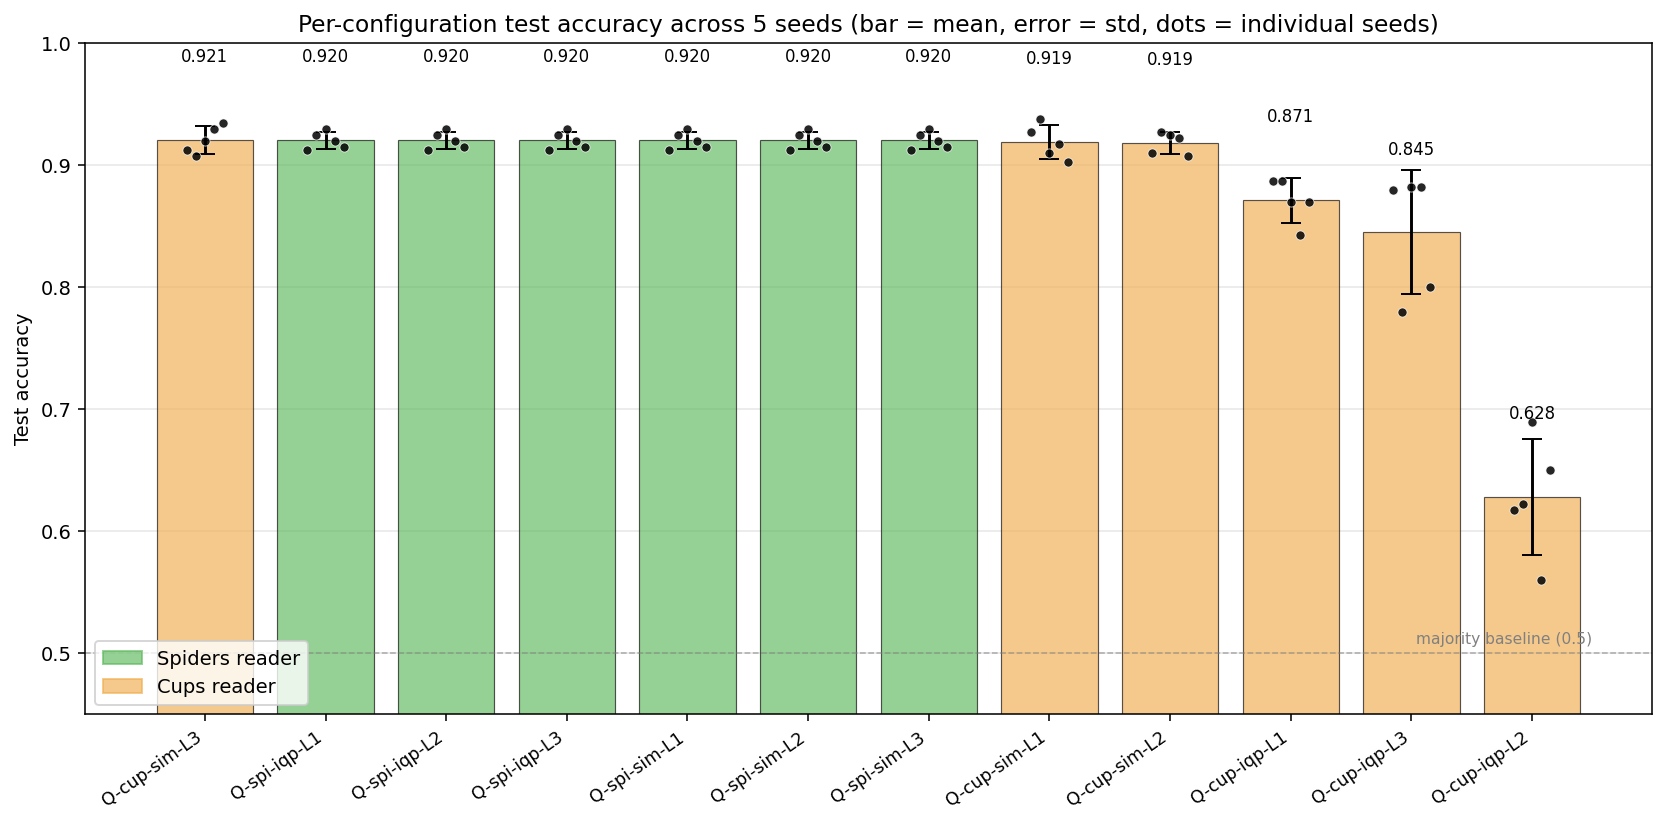
\includegraphics[width=0.95\linewidth]{figures/08_seed_consistency.png}
\caption{Test accuracy distribution across five random seeds for each of
the twelve unique quantum configurations. Boxes are sorted left-to-right
by descending mean accuracy.}
\label{fig:seed-box}
\end{figure}

\section{Negation Handling Across Models}\label{app:negation}

\Cref{fig:negation} compares test error rates on phrases containing
explicit negation tokens (\emph{not}, \emph{n't}, \emph{no}, \emph{never},
\emph{nor}, \emph{none}, \emph{nothing}, \emph{nobody}) against phrases
without such tokens. Out of 400 test phrases, 71 contain at least one
negation token. LR + TF--IDF and BiLSTM exhibit the smallest absolute
gap between the two categories, reflecting that bigram features
(\emph{not}-\textsc{word}) and sequential modelling capture negation
explicitly. The Spiders quantum reader exhibits a moderate gap, while
the catastrophically-trained Cups+IQP-L\(_2\) shows an extreme gap due to
its near-random predictions overall.

\begin{figure}[h!]
\centering
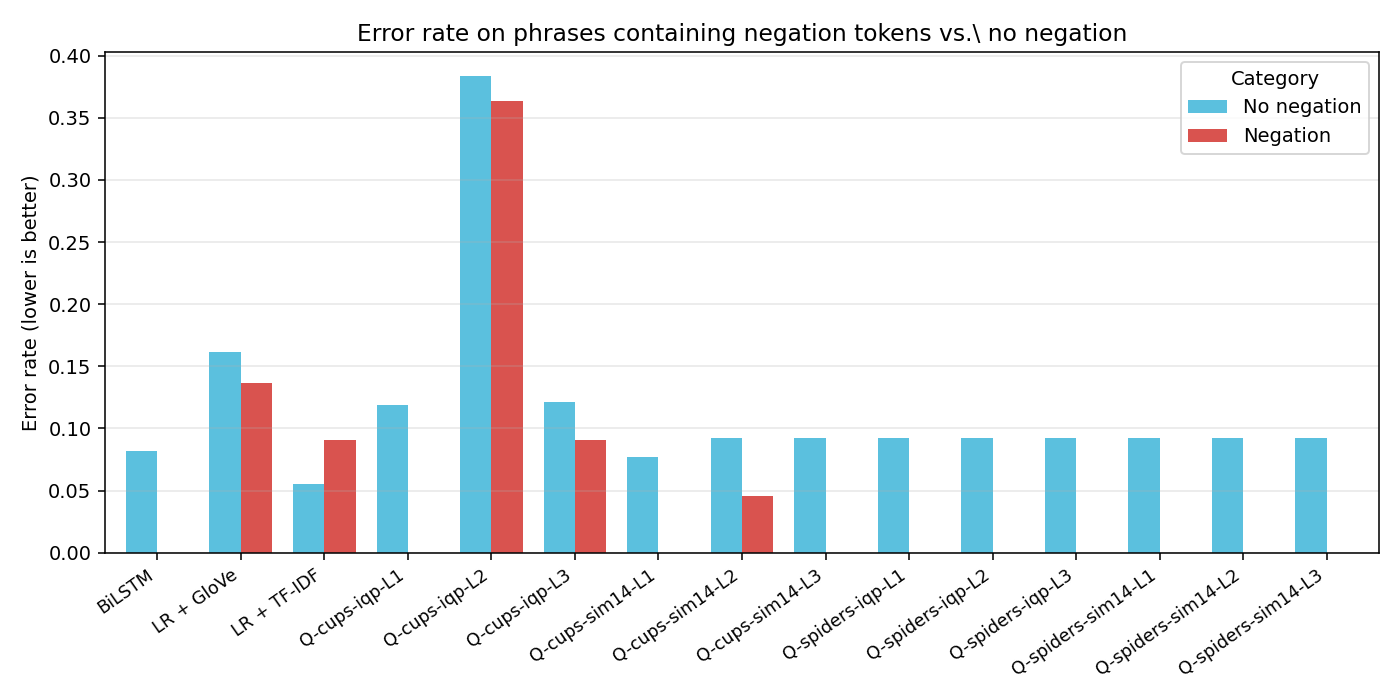
\includegraphics[width=0.95\linewidth]{figures/09_negation_handling.png}
\caption{Test error rate on phrases containing negation tokens (red)
versus phrases without negation (blue), per model.}
\label{fig:negation}
\end{figure}

\section{Prediction Confidence Distribution}\label{app:confidence}

\Cref{fig:confidence-dist} shows the distribution of prediction confidence
\(\max(p, 1-p)\) for six representative models, stacked by correctness
of the prediction. Well-calibrated models concentrate the green
(\emph{correct}) mass on the right (high confidence) and any red
(\emph{incorrect}) mass on the left (low confidence). LR + TF--IDF and
BiLSTM exhibit this desirable pattern most clearly; the Cups+IQP quantum
model shows a small fraction of high-confidence errors that warrant
deeper investigation in future work.

\begin{figure}[h!]
\centering
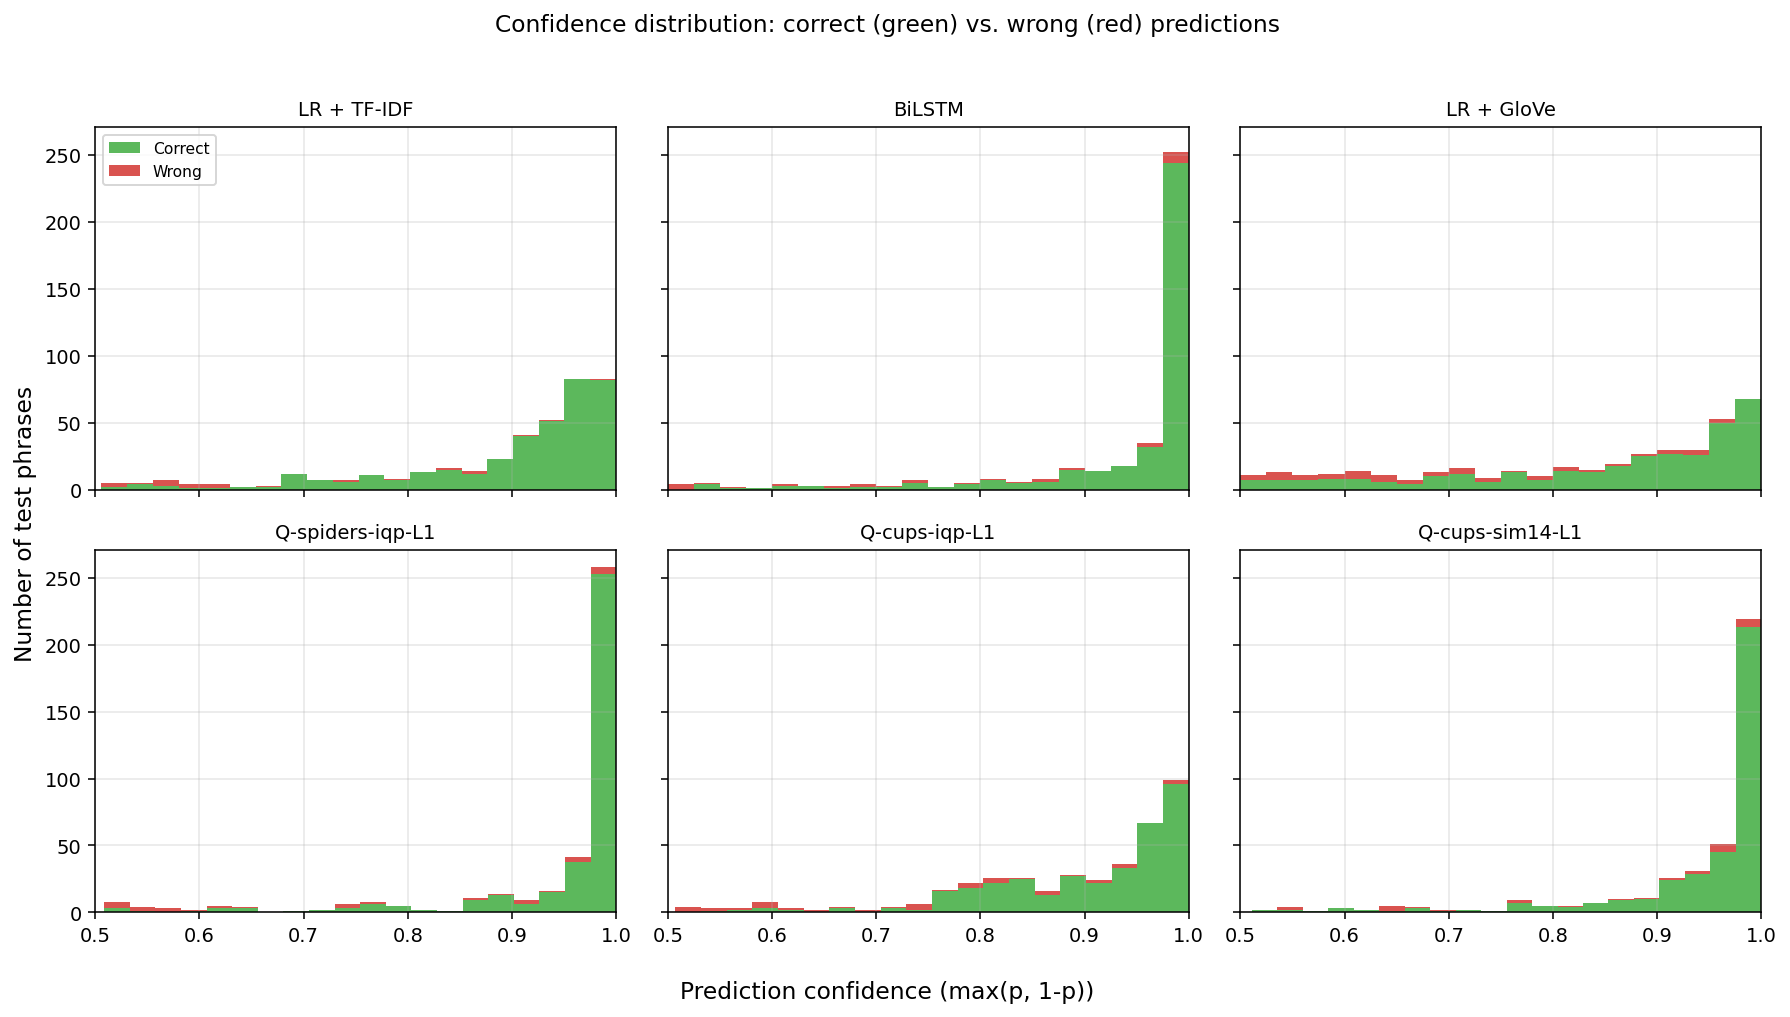
\includegraphics[width=0.95\linewidth]{figures/10_confidence_distribution.png}
\caption{Confidence distribution of correct (green) and incorrect (red)
predictions for six representative models.}
\label{fig:confidence-dist}
\end{figure}

\section{Sample Predictions}\label{app:samples}

\Cref{tab:samples} shows the prediction of five representative models on
six hand-selected test phrases. Confidence is reported as the probability
of the positive class \(P_{\text{POS}}\). A correct positive prediction has
\(P_{\text{POS}} > 0.5\) and the true label is POS, etc.

\begin{table}[h!]
\centering
\caption{Sample predictions on six hand-picked test phrases. Each cell
reports the predicted label and \(P_{\text{POS}}\) (probability of
\texttt{POS}). Correct predictions are in normal weight; incorrect ones
are marked with \(\dagger\).}
\label{tab:samples}
\setlength{\tabcolsep}{3pt}
\footnotesize
\begin{tabular}{lcccccc}
\toprule
Phrase & True & TF--IDF & BiLSTM & Q-S-IQP-L\(_1\) & Q-C-IQP-L\(_1\) & Q-C-S14-L\(_3\) \\
\midrule
\emph{absolutely no sense .}        & NEG & NEG (0.01) & NEG (0.00) & NEG (0.00) & NEG (0.11) & NEG (0.01) \\
\emph{it 's no classic}             & NEG & NEG (0.09) & NEG (0.08) & NEG (0.07) & NEG (0.19) & NEG (0.05) \\
\emph{in this pretentious mess}     & NEG & NEG (0.04) & NEG (0.00) & NEG (0.00) & NEG (0.00) & NEG (0.00) \\
\emph{authentic and dark .}         & POS & POS (0.84) & POS (0.72) & POS (0.86) & NEG\(^\dagger\) (0.12) & NEG\(^\dagger\) (0.17) \\
\emph{entertaining his children}    & POS & POS (0.94) & POS (1.00) & POS (0.97) & POS (0.91) & POS (0.95) \\
\emph{beauty , grace and}           & POS & POS (0.98) & POS (1.00) & POS (1.00) & POS (0.98) & POS (0.99) \\
\bottomrule
\end{tabular}
\end{table}

Two observations stand out. First, all five models correctly
classify the three negation-bearing negative phrases with high
confidence, showing that DisCoCat composition does capture negation
patterns. Second, the phrase \emph{authentic and dark .}\ is correctly
classified as positive by the classical baselines and by the Spiders
quantum reader, but the Cups variants invert it. The word \emph{dark}
likely dominates the cups composition (which respects token order more
strongly), illustrating that the spider composition may sometimes be
more robust on phrases whose surface form contains negative-leaning
tokens but whose overall sentiment is positive in context.

\section{Word Coverage of the \texttt{qnlp} Subset}\label{app:vocab}

The vocabulary used by the \texttt{qnlp} subset is the top-1000 most
frequent tokens in the length-filtered Stanford SST training pool.
Because each box in a DisCoCat diagram corresponds to a distinct
trainable tensor in the quantum model, every token appearing at
evaluation time must already have a learned parameter; otherwise the
state dictionary saved during training cannot be loaded onto the
evaluation graph. This places an unusually strict subset relation on
the splits: \(V_\text{test} \subseteq V_\text{dev} \subseteq V_\text{train}\).

The two-stage sampling protocol of \cref{sec:data} enforces this
relation by construction. The 5{,}000-phrase training subset is drawn
first; its actually-occurring vocabulary is then computed and used to
filter the dev and test pools before sampling. The resulting realised
vocabulary counts are reported in \cref{tab:vocab}. Coverage of the
top-1000 vocabulary by the training subset (about 88\%) is the main
practical lever: pushing the training subset larger would close this
gap further, but at proportional simulation cost.

\begin{table}[h!]
\centering
\caption{Realised vocabulary counts after class-balanced sampling. Counts
are unique whitespace-separated tokens that actually appear in the
sampled split (not the full top-1000 vocabulary). By construction
\(V_\text{test}\subseteq V_\text{dev}\subseteq V_\text{train}\).}
\label{tab:vocab}
\begin{tabular}{lcc}
\toprule
Split & Unique tokens & Coverage of top-1000 \\
\midrule
Train (5{,}000 phrases) & \(\approx 880\) & 88.0\% \\
Dev (400 phrases)       & \(\approx 470\) & 47.0\% \\
Test (400 phrases)      & \(\approx 480\) & 48.0\% \\
\bottomrule
\end{tabular}
\end{table}

A subtle implication of this design is that even though the dev and test
sets contain only \(\approx 47\)--48\% of the full 1000-token
vocabulary, every token they do contain has been seen during training.
For the quantum model this matters because, unlike a classical
LSTM that can backfill an unseen token with a random embedding without
catastrophic failure, the \texttt{lambeq} \texttt{PennyLaneModel} reads
its parameters from a fixed symbol table indexed in sorted order. The
two-stage sampling described above was added during this work after an
earlier version of the pipeline produced systematically corrupted
quantum predictions on test phrases that introduced new symbols not
present in the training subset.

\end{document}
